\documentclass[letterpaper,10pt]{article}

\usepackage{tabularx} % extra features for tabular environment
\usepackage{amsmath}  % improve math presentation
\usepackage{graphicx} % takes care of graphic including machinery
\usepackage[margin=1in,letterpaper]{geometry} % decreases margins
\usepackage{cite} % takes care of citations
\usepackage[final]{hyperref} % adds hyper links inside the generated pdf file
\usepackage{ctex}
\usepackage{titlesec}
%\usepackage{CJKutf8, CJK}
\usepackage{makecell}                 % 三线表-竖线
\usepackage{booktabs}                 % 三线表-短细横线
% \usepackage{natbib}
\usepackage{graphicx}				  % 表格单元格逆时针
\usepackage{multirow}				  % 合并单元格
\usepackage{array}
\usepackage{amssymb}				  % 勾
\usepackage{amsmath}
\usepackage{longtable}                % 导入 longtable 宏包,表格自动换行
\usepackage{caption}
\usepackage{subcaption}               % 设置子图
\usepackage{color}					  % 文本颜色包
\usepackage{xcolor}
\usepackage{bbm}					  % 输入指示函数
\usepackage{tablefootnote}			  % 表格注释
\usepackage{pythonhighlight}
\usepackage{fancyhdr}
\usepackage{lastpage}
\pagestyle{fancy}
\fancyhf{}
\fancyhead{}
\fancyfoot{}
\fancyhead[R]{\small Page \thepage\ of \pageref*{LastPage}}
\fancyhead[L]{\small Report}

\usepackage{listings}                 % 导入代码块
\usepackage{xcolor}
\lstset{
	numbers=left, 
	tabsize=1,
	columns=flexible, 
	numberstyle=  \small, 
	keywordstyle= \color{ blue!70},
	commentstyle= \color{red!50!green!50!blue!50}, 
	frame=shadowbox, % 阴影效果
	rulesepcolor= \color{ red!20!green!20!blue!20} ,
	escapeinside=``, % 英文分号中可写入中文
	xleftmargin=2em,
	xrightmargin=2em, 
	aboveskip=1em,
} 

\hypersetup{
	colorlinks=true,       % false: boxed links; true: colored links
	linkcolor=blue,        % color of internal links
	citecolor=blue,        % color of links to bibliography
	filecolor=magenta,     % color of file links
	urlcolor=blue         
}
%++++++++++++++++++++++++++++++++++++++++
\titleformat{\section}{\Large\bfseries\songti}{\thesection}{1em}{}
\titleformat{\subsection}{\large\bfseries\songti}{\thesubsection}{1em}{}
\titleformat{\subsubsection}{\normalsize\bfseries\songti}{\thesubsubsection}{1em}{}
\titleformat{\paragraph}{\small\bfseries\songti}{\paragraph}{1em}{}
\titleformat{\subparagraph}{\footnotesize\bfseries\songti}{\subparagraph}{1em}{}

\begin{document}
	
	
	\title{\songti \zihao{4}8月30日-9月5日工作汇报}
	\author{\textrm{Ku Jui}}
	\date{\textrm{September 2023}}
	\maketitle
	
	\renewcommand{\figurename}{Figure} % 可以重新定义abstract,因为ctex会覆盖thebibliography
	% 	\begin{abstract}
		%		In this experiment we studied a very important physical effect by measuring the
		%		dependence of a quantity $V$ of the quantity $X$ for two different sample
		%		temperatures.  Our experimental measurements confirmed the quadratic dependence
		%		$V = kX^2$ predicted by Someone's first law. The value of the mystery parameter
		%		$k = 15.4\pm 0.5$~s was extracted from the fit. This value is
		%		not consistent with the theoretically predicted $k_{theory}=17.34$~s. We attribute %this
		%		discrepancy to low efficiency of our $V$-detector.
		%	\end{abstract}
	\renewcommand{\contentsname}{Contents}
	\renewcommand{\tablename}{Table}
	\tableofcontents  % 自动生成目录
	
	\part{Pre-Knowledge}	

	
	
%%%%%%%%%%%%%%%%%%%%%%%%%%%%%%%%%%%%%%%%%%%%%%%%%%%%%%%%%%%%%%%%%%%%%%%%%%%%%%%%%%%%%%%%%%%%%%%%%%%%
%%%%%%%%%%%%%%%%%%%%%%%%%%%%%%%%%%%%%%%%%%%%%%%%%%%%%%%%%%%%%%%%%%%%%%%%%%%%%%%%%%%%%%%%%%%%%%%%%%%%
%%                                                                                                %% 
%%								          Paper reading                                           %%
%%                                                                                                %%
%%%%%%%%%%%%%%%%%%%%%%%%%%%%%%%%%%%%%%%%%%%%%%%%%%%%%%%%%%%%%%%%%%%%%%%%%%%%%%%%%%%%%%%%%%%%%%%%%%%%
%%%%%%%%%%%%%%%%%%%%%%%%%%%%%%%%%%%%%%%%%%%%%%%%%%%%%%%%%%%%%%%%%%%%%%%%%%%%%%%%%%%%%%%%%%%%%%%%%%%%	

	
	\part{Paper Reading}
	
	\section{LLIE}
	
		\subsection{(2023.1)Illumination estimation for nature preserving low-light image enhancement}
		
		\paragraph{低光图像增强中保留自然光的照度估计}
		
		\paragraph{(The Visual Computer 3区) doi: 10.1007/s00371-023-02770-9}
		
			\subsubsection{Research Background}
			
			在 Retinex 模型\footnote{Retinex 模型的理论基础是三色理论和颜色恒常性:即物体的颜色是由物体对长波(红色)、中波(绿色)、短波(蓝色)光线的反射能力来决定的,而不是由反射光强度的绝对值来决定的,物体的色彩不受光照非均匀性的影响,具有一致性,即 Retinex 是以色感一致性(颜色恒常性)为基础的。}中,图像被认为是两个组成部分的组合:照度 (illumination) 和反射率 (reflectance)。但是,将图像分解为照度和反射率是一个不适定的问题\footnote{Retinex 模型认为图像 $\mathcal{I}(x,y)$ 由照度图像 $\mathcal{L}(x,y)$ 与反射图像 $\mathcal{R}(x,y)$ 组成。前者指的是物体的入射分量的信息,用 $\mathcal{L}(x,y)$ 表示;后者指的是物体的反射部分,用 $\mathcal{R}(x,y)$ 表示。公式:$\mathcal{I}(x,y)=\mathcal{R}(x,y) \cdot \mathcal{L}(x,y)$。}\footnote{将图像分解为照度和反射率是一个不适定问题,因为它不满足适定性问题的三个条件之一或几个。适定性问题是指定解满足下面三个要求的问题:解是存在的;解是唯一的;解连续依赖于定解条件,即解是稳定的。如果不满足这些条件,则称之为不适定问题。这意味着即使输入图像只有微小的变化,输出的照度和反射率也可能会发生巨大的变化。举个例子,假设我们有一张图像,它的某个像素点的颜色值为(100,100,100),我们可以通过某种算法将其分解为照度和反射率两个部分。但是,如果我们将这个像素点的颜色值稍微改变一下,比如变为(101,101,101),那么输出的照度和反射率可能会发生巨大的变化。}。一般来说,基于 Retinex 模型的方法在亮度增强和自然度保持之间存在权衡,即如果算法保持自然度,则整体亮度较低,反之亦然。
		
			\subsubsection{Contribution}
			
			作者提出了一种估计弱光图像增强照度的新方法。即利用一种新的多尺度引导滤波方法提出了一种结构感知初始照明估计的新方法,主要包括以下三个任务:
			
			\begin{itemize}
				\item[(1)] 
				结构感知初始照度\footnote{在 Retinex 算法中,可以通过对原始图像进行高斯滤波来获取照度图像,并尽量准确地获取照度图像,最后将照度图像从原始图像中分离出来,从而获得反射图像。分离过程可以通过对数与反对数 Map 以及图像拉伸算法来实现。}的估计;
				
				\item[(2)]
				估计照度的细化;
				
				\item[(3)]
				细化照度的最终校正。
			\end{itemize}	
			
			此外,作者提出了一种新的自适应照度调整方法,利用估计的照度对亮度进行校正。
			
			\subsubsection{Approach}
			
			作者的方法主要估计图像的照度,并利用 Retinex 模型获得反射分量。
			
			\begin{itemize}
				\item[(1)] 
				首先,其使用在引导滤波器中提出的多个框(窗口)大小来估计结构感知的初始照度;
				
				\item[(2)]
				然后,作者通过构造和求解一个新的多目标优化函数来细化初始照度;
				
				\item[(3)]
				最后作者应用提出的自适应照度调整,在估计照度的基础上提高图像的亮度。
			\end{itemize}	
			
			\subsubsection{Future}
			
			- 
		
		\subsection{(2023.7)Division Gets Better: Learning Brightness-Aware and Detail-Sensitive Representations for Low-Light Image Enhancement}
		
		\paragraph{分割可以变得更好:学习亮度感知和细节敏感的表示为低光图像增强}
		
		\paragraph{(CVPR 2023) doi: 10.48550/arXiv.2307.09104}
		
			\subsubsection{Research Background}
			
			现有的方法通常更注重通过增加低照度图像的亮度来提高图像的可见度和对比度,而忽略了高质量图像的色彩和纹理恢复的重要性。
			
		    以往的方法通常在 RGB 空间操作,这导致设计的模型很难通过单个 CNN 同时学习亮度特征和细节特征(包括纹理和颜色)。同时新的解决方法产生的视觉结果,无法代表自然图像的局部颜色变化。
			
			\begin{figure}[htbp] 
				% read manual to see what [ht] means and for other possible options
				\centering 
				% 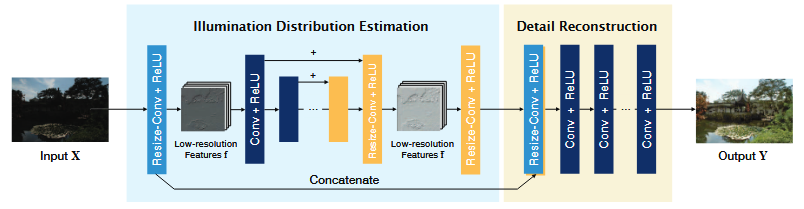
\includegraphics[width=0.8\columnwidth]{GLADNet}
				
				\begin{subfigure}{0.11\textwidth}
					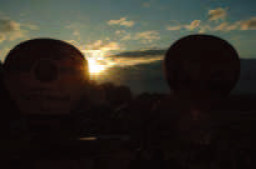
\includegraphics[width=\linewidth]{picture/LLIE/Division Gets Better/RGB-low light1}
					\captionsetup{font=scriptsize}
					\label{fig: RGB-low light1}
				\end{subfigure}
				\begin{subfigure}{0.11\textwidth}
					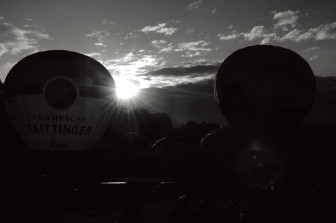
\includegraphics[width=\linewidth]{picture/LLIE/Division Gets Better/R1}
					\captionsetup{font=scriptsize}
					\label{fig: R1}
				\end{subfigure}
				\begin{subfigure}{0.11\textwidth}
					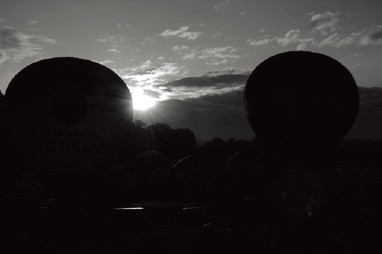
\includegraphics[width=\linewidth]{picture/LLIE/Division Gets Better/G1}
					\captionsetup{font=scriptsize}
					\label{fig: G1}	
				\end{subfigure}
				\begin{subfigure}{0.11\textwidth}
					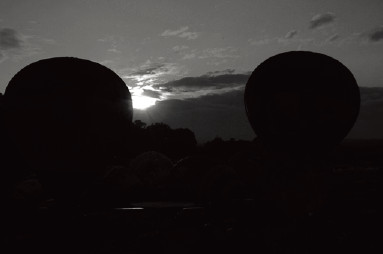
\includegraphics[width=\linewidth]{picture/LLIE/Division Gets Better/B1}
					\captionsetup{font=scriptsize}
					\label{fig: B1}	
				\end{subfigure}
				\begin{subfigure}{0.11\textwidth}
					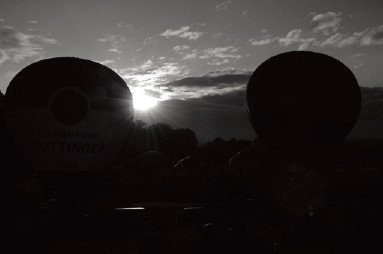
\includegraphics[width=\linewidth]{picture/LLIE/Division Gets Better/Y1}
					\captionsetup{font=scriptsize}
					\label{fig: Y1}	
				\end{subfigure}
				\begin{subfigure}{0.11\textwidth}
					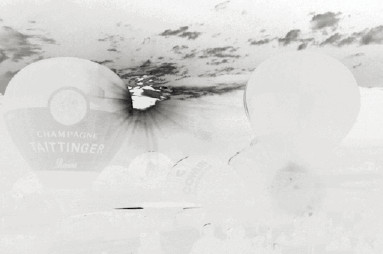
\includegraphics[width=\linewidth]{picture/LLIE/Division Gets Better/Cb1}
					\captionsetup{font=scriptsize}
					\label{fig: Cb1}	
				\end{subfigure}
				\begin{subfigure}{0.11\textwidth}
					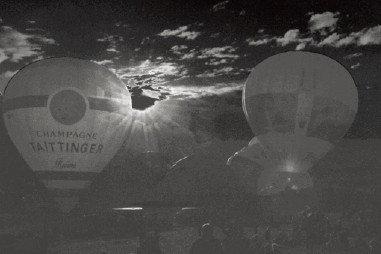
\includegraphics[width=\linewidth]{picture/LLIE/Division Gets Better/Cr1}
					\captionsetup{font=scriptsize}
					\label{fig: Cr1}	
				\end{subfigure}
				\begin{subfigure}{0.11\textwidth}
					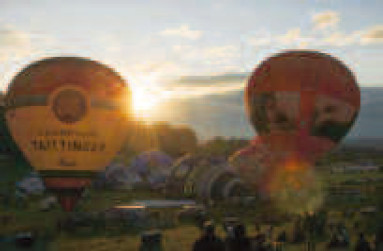
\includegraphics[width=\linewidth]{picture/LLIE/Division Gets Better/Ours1}
					\captionsetup{font=scriptsize}
					\label{fig: Ours1}	
				\end{subfigure}\\
				
				\begin{subfigure}{0.11\textwidth}
					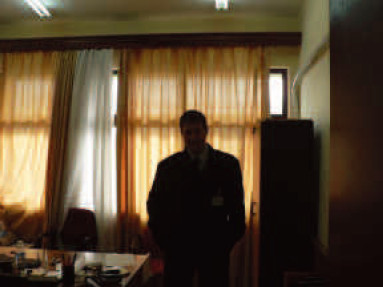
\includegraphics[width=\linewidth]{picture/LLIE/Division Gets Better/RGB-low light2}
					\captionsetup{font=scriptsize}
					\label{fig: RGB-low light2}
				\end{subfigure}
				\begin{subfigure}{0.11\textwidth}
					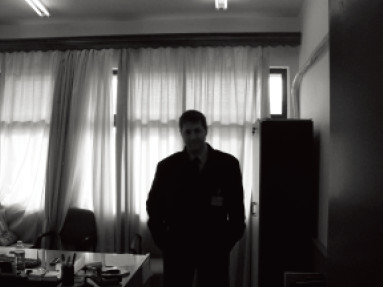
\includegraphics[width=\linewidth]{picture/LLIE/Division Gets Better/R2}
					\captionsetup{font=scriptsize}
					\label{fig: R2}
				\end{subfigure}
				\begin{subfigure}{0.11\textwidth}
					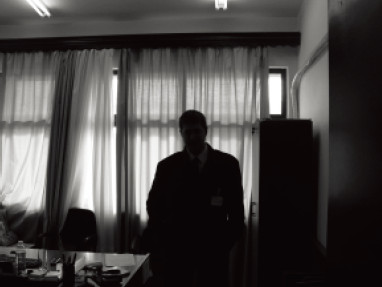
\includegraphics[width=\linewidth]{picture/LLIE/Division Gets Better/G2}
					\captionsetup{font=scriptsize}
					\label{fig: G2}
				\end{subfigure}
				\begin{subfigure}{0.11\textwidth}
					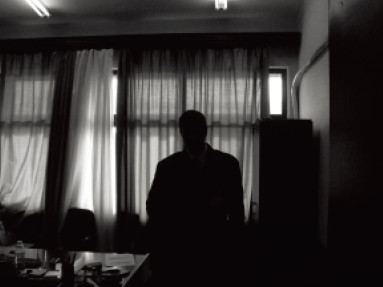
\includegraphics[width=\linewidth]{picture/LLIE/Division Gets Better/B2}
					\captionsetup{font=scriptsize}
					\label{fig: B2}	
				\end{subfigure}
				\begin{subfigure}{0.11\textwidth}
					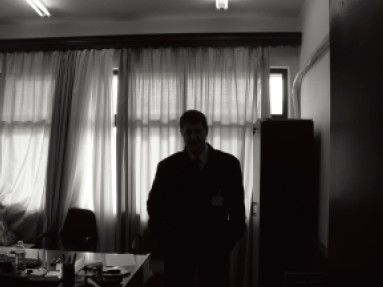
\includegraphics[width=\linewidth]{picture/LLIE/Division Gets Better/Y2}
					\captionsetup{font=scriptsize}
					\label{fig: Y2}	
				\end{subfigure}
				\begin{subfigure}{0.11\textwidth}
					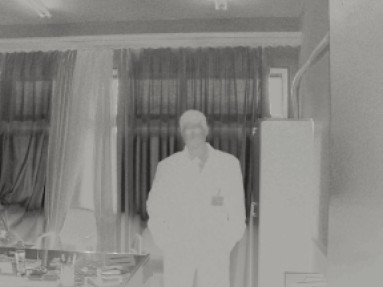
\includegraphics[width=\linewidth]{picture/LLIE/Division Gets Better/Cb2}
					\captionsetup{font=scriptsize}
					\label{fig: Cb2}	
				\end{subfigure}
				\begin{subfigure}{0.11\textwidth}
					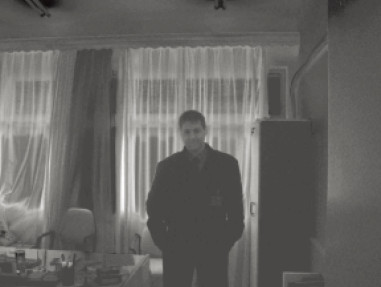
\includegraphics[width=\linewidth]{picture/LLIE/Division Gets Better/Cr2}
					\captionsetup{font=scriptsize}
					\label{fig: Cr2}	
				\end{subfigure}
				\begin{subfigure}{0.11\textwidth}
					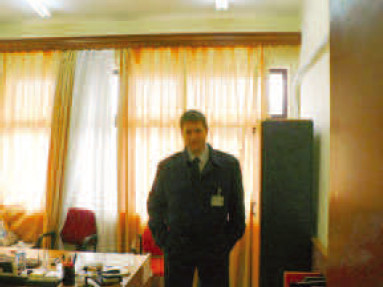
\includegraphics[width=\linewidth]{picture/LLIE/Division Gets Better/Ours2}
					\captionsetup{font=scriptsize}
					\label{fig: Ours2}	
				\end{subfigure}\\
				
				\begin{subfigure}{0.11\textwidth}
					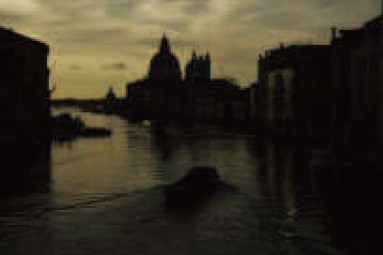
\includegraphics[width=\linewidth]{picture/LLIE/Division Gets Better/RGB-low light3}
					\captionsetup{font=scriptsize}
					\caption*{RGB-low light}
					\label{fig: RGB-low light3}
				\end{subfigure}
				\begin{subfigure}{0.11\textwidth}
					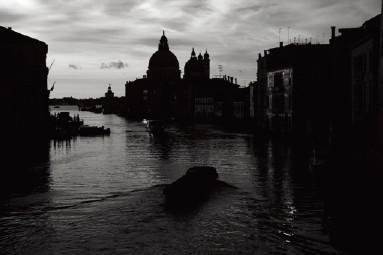
\includegraphics[width=\linewidth]{picture/LLIE/Division Gets Better/R3}
					\captionsetup{font=scriptsize}
					\caption*{R}
					\label{fig: R3}
				\end{subfigure}
				\begin{subfigure}{0.11\textwidth}
					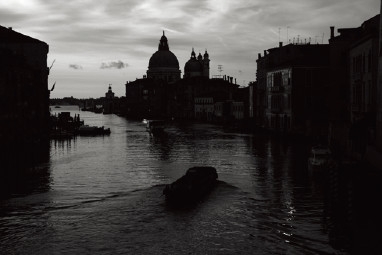
\includegraphics[width=\linewidth]{picture/LLIE/Division Gets Better/G3}
					\captionsetup{font=scriptsize}
					\caption*{G}
					\label{fig: G3}
				\end{subfigure}
				\begin{subfigure}{0.11\textwidth}
					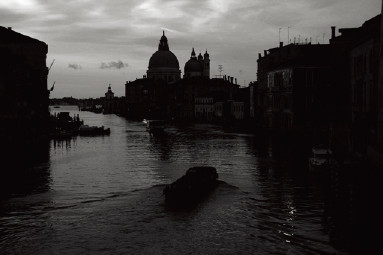
\includegraphics[width=\linewidth]{picture/LLIE/Division Gets Better/B3}
					\captionsetup{font=scriptsize}
					\caption*{B}
					\label{fig: B3}
				\end{subfigure}
				\begin{subfigure}{0.11\textwidth}
					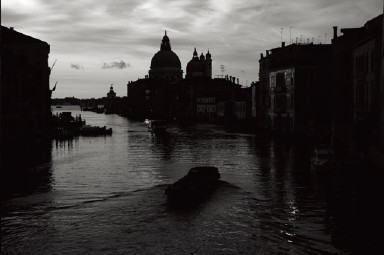
\includegraphics[width=\linewidth]{picture/LLIE/Division Gets Better/Y3}
					\captionsetup{font=scriptsize}
					\caption*{Y}
					\label{fig: Y3}
				\end{subfigure}
				\begin{subfigure}{0.11\textwidth}
					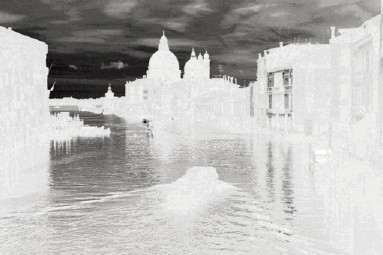
\includegraphics[width=\linewidth]{picture/LLIE/Division Gets Better/Cb3}
					\captionsetup{font=scriptsize}
					\caption*{Cb}
					\label{fig: Cb3}
				\end{subfigure}
				\begin{subfigure}{0.11\textwidth}
					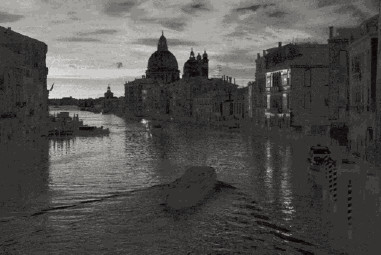
\includegraphics[width=\linewidth]{picture/LLIE/Division Gets Better/Cr3}
					\captionsetup{font=scriptsize}
					\caption*{Cr}
					\label{fig: Cr3}
				\end{subfigure}
				\begin{subfigure}{0.11\textwidth}
					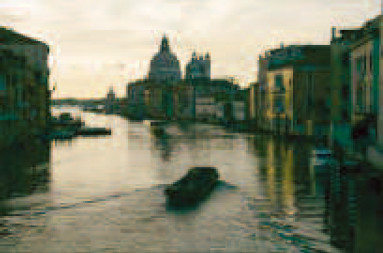
\includegraphics[width=\linewidth]{picture/LLIE/Division Gets Better/Ours3}
					\captionsetup{font=scriptsize}
					\caption*{Ours}
					\label{fig: Our3}
				\end{subfigure}
				\captionsetup{font=scriptsize}
				\caption{
					\label{fig: Low-light images and their luminance and chrominance decomposition}
					Low-light images and their luminance and chrominance decomposition. The first four columns show original low-light images in
					RGB space and their RGB channel decomposition, the fifth column shows luminance (Y) channels of low-light images, the sixth and seventh
					columns are chrominance (CbCr) components of low-light images, and the last column exhibits the enhanced images by our method. We
					can obviously observe that three channels of RGB space indicate indistinguishable distortion patterns, and Y and CbCr components reveal
					distinctly different distortion patterns.
				}
			\end{figure}
			
			\subsubsection{Contribution}
			
			针对上述问题,本文提出了一种用于微光图像增强的亮度和色度双分支网络 LCDBNet,该网络将微光图像增强分为亮度调整和色度恢复两个子任务。
			
			\begin{itemize}
				\item[(1)] 
				LCDBNet 由两个分支组成,即亮度调整网络 (LAN) 和亮度恢复网络 (CRN)。
				
				\item[(2)]
				LAN 负责学习利用远程依赖和局部注意关联的亮度感知特性。
				
				\item[(3)]
				CRN 则专注于通过多级小波分解学习细节敏感特征。
				
				\item[(4)]
				最后,设计了一个融合网络,将学习到的特征融合在一起,产生令人印象深刻的视觉图像。
			\end{itemize}	
			
			\subsubsection{Approach}
			
			开发了一个全局和局部聚合块 (GLAB) 作为 LAN 的构建块,如 Fig. \ref{fig: LCDBNet},它由一个 Transformer 分支和一个双注意卷积块 (DACB) 组成,用于学习非局部表示和局部信息。
			
			为了恢复图像细节,引入小波变换辅助 CRN 提取高频细节信息。
			
			网络由亮度调节网络 (LAN) 和色度恢复网络 (CRN) 两个子网络组成。利用 LAN 从亮度通道中获取亮度感知特征,利用 CRN 从亮度通道中提取细节敏感特征。
			
			\begin{figure}[htbp]
				% read manual to see what [ht] means and for other possible options
				\centering 
				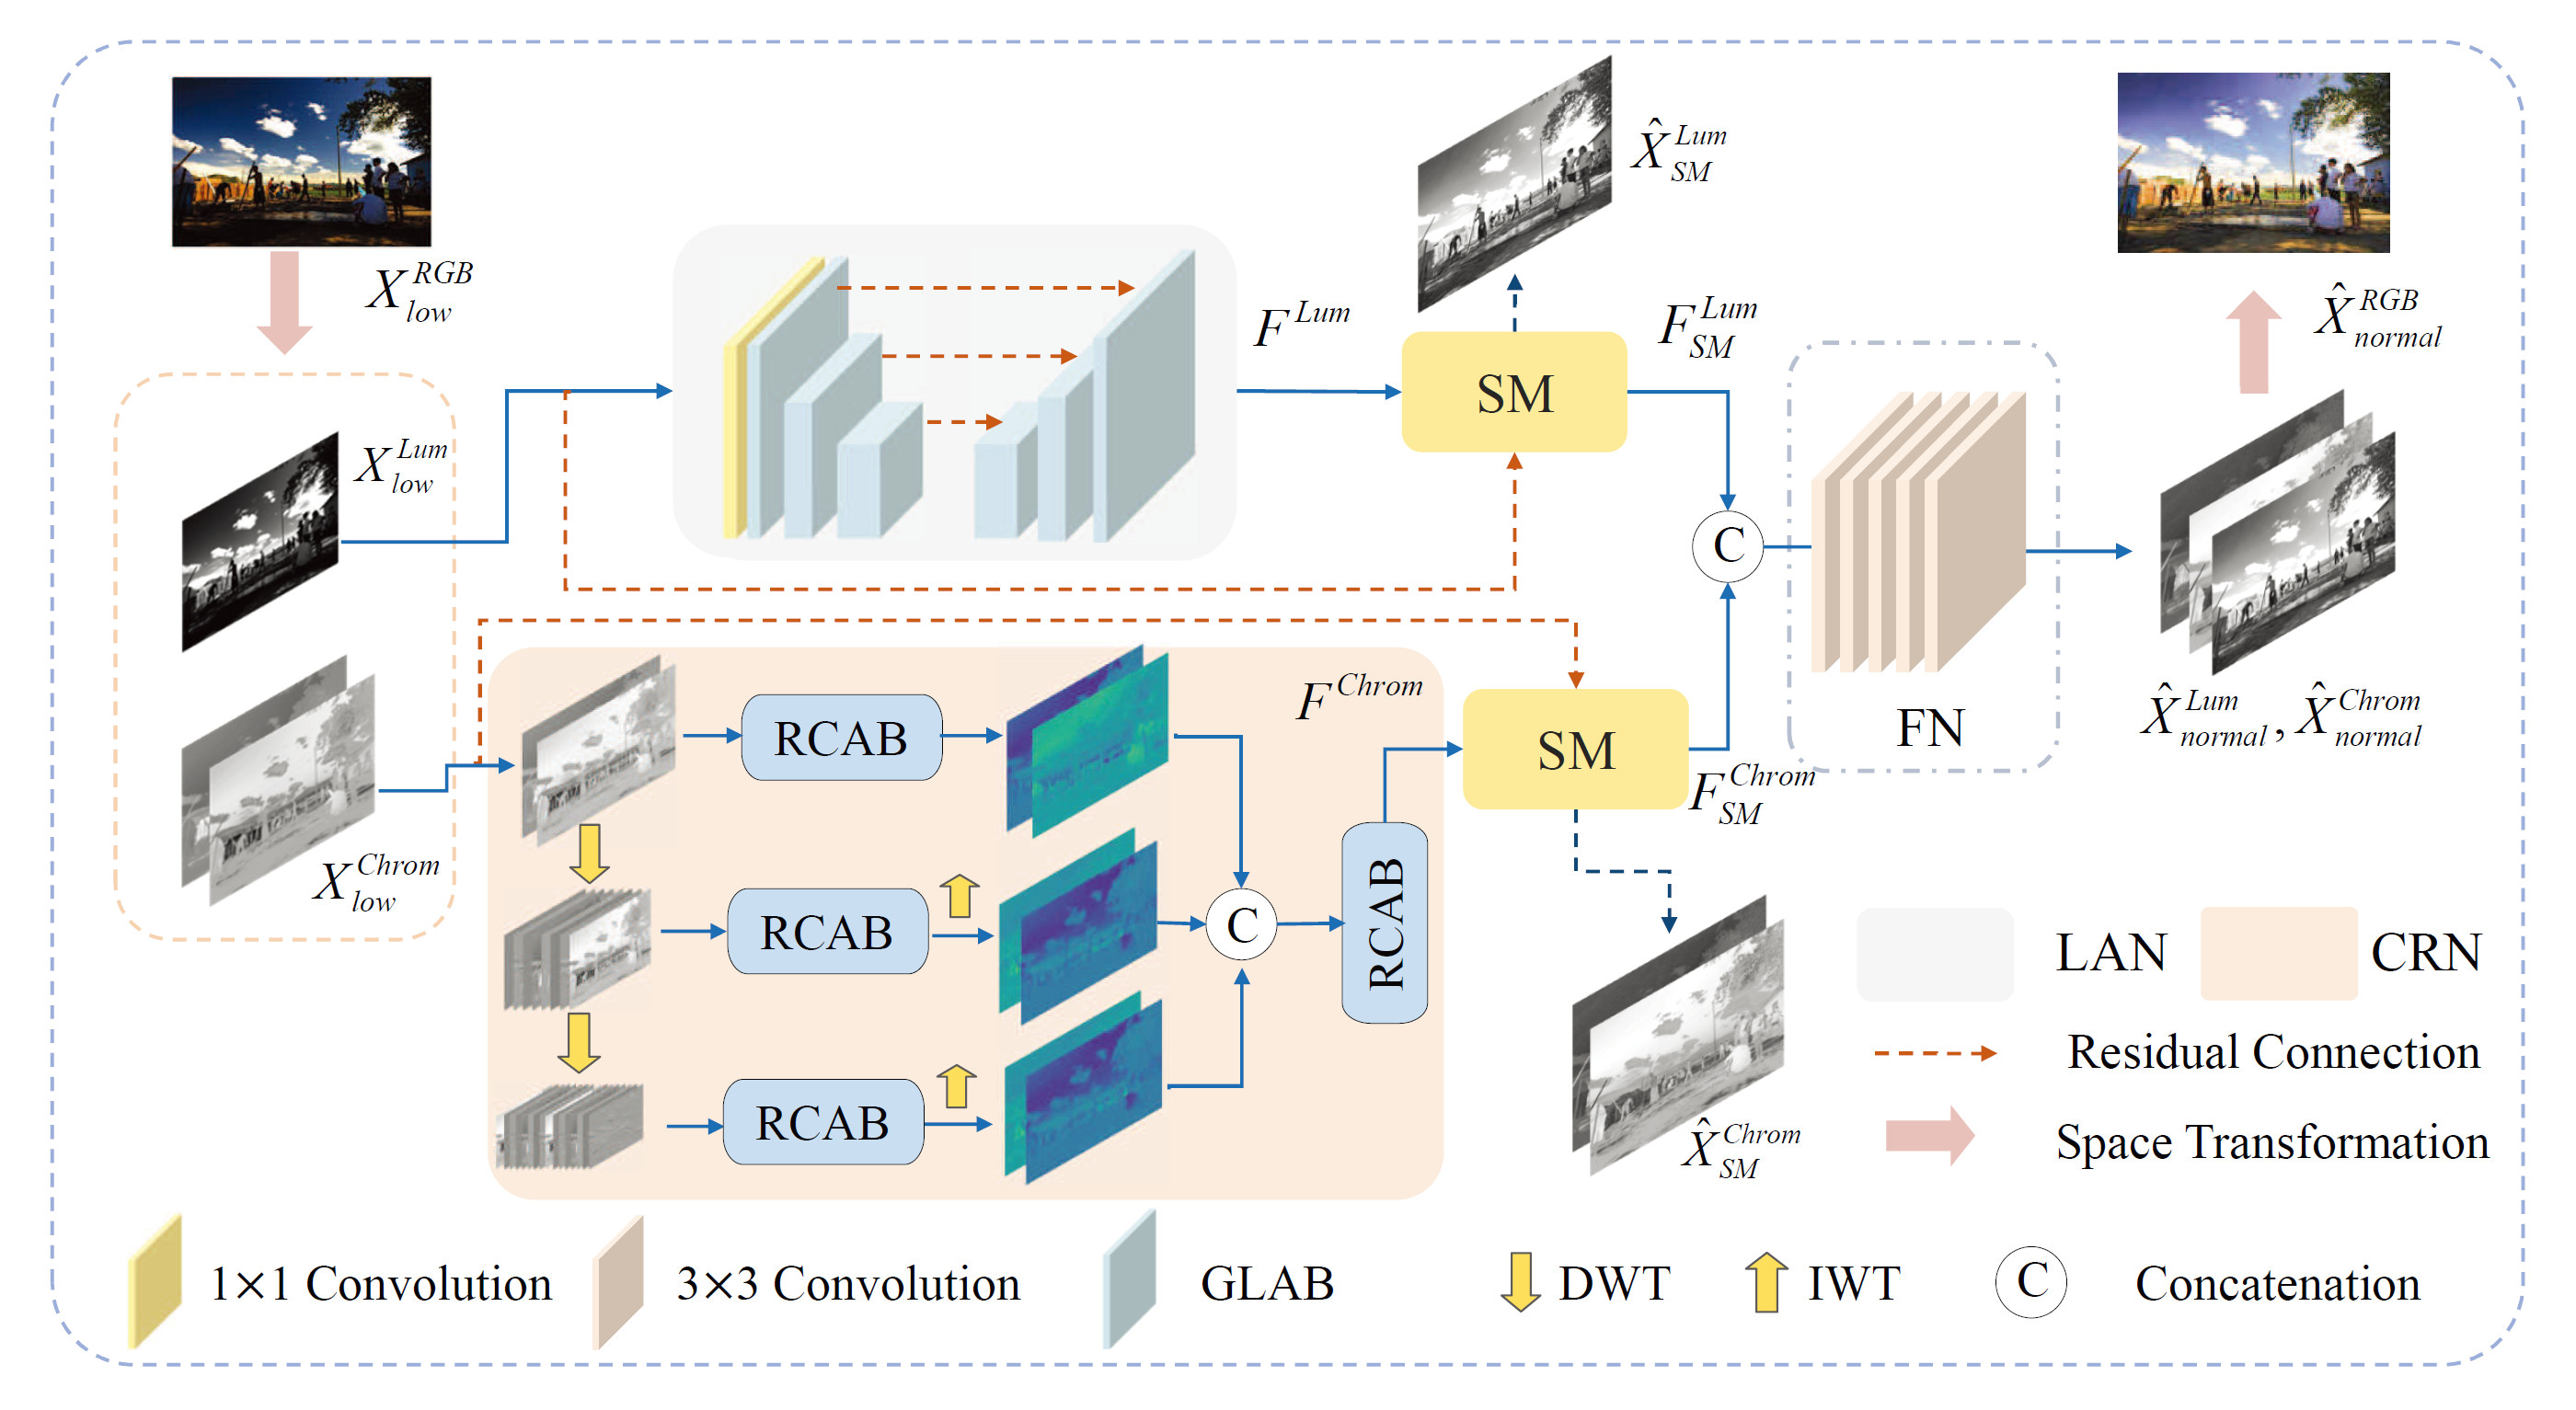
\includegraphics[width=\columnwidth]{picture/LLIE/LCDBNet}
				%\captionsetup{font=scriptsize}
				\caption{
					\label{fig: LCDBNet} 
					The overview of the proposed LCDBNet. The input images are transformed from RGB space to YCbCr space. Luminance and
					chrominance components are fed into LAN and CRN, respectively. Then, their outputs are fused in FN to derive the enhanced results.
					Finally, the enhanced images are converted back to RGB space.
				}
			\end{figure}
			
			\subsubsection{Future}
		
			-
			
		\subsection{(2023.3)Advanced RetinexNet: A fully convolutional network for low-light image enhancement}
			
		\paragraph{Advanced RetinexNet:用于弱光图像增强的全卷积网络}
			
		\paragraph{(Signal Processing: Image Communication 二区) doi: 10.1016/j.image.2022.116916}
			
			\subsubsection{Research Background}
				
			以往的方法在提高图像对比度方面取得很大的进步,但大多数方法都不能很好地增强图像对比度,结果往往是增强不足或噪声放大。如Fig. \ref{fig: Examples of LLIE}所示。
				
			\begin{figure}[htbp] 
				% read manual to see what [ht] means and for other possible options
				\centering 
				% 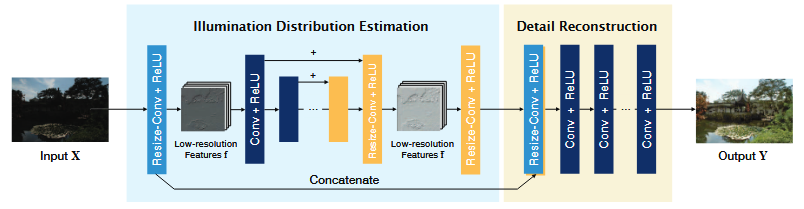
\includegraphics[width=0.8\columnwidth]{GLADNet}
				
				\begin{subfigure}{0.24\textwidth}
					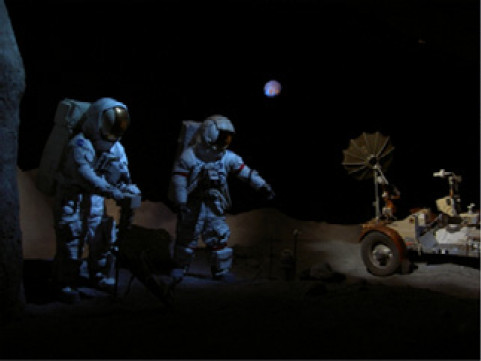
\includegraphics[width=\linewidth]{picture/LLIE/Input1}
					\captionsetup{font=scriptsize}
					\label{fig: Input1}
				\end{subfigure}
				\begin{subfigure}{0.24\textwidth}
					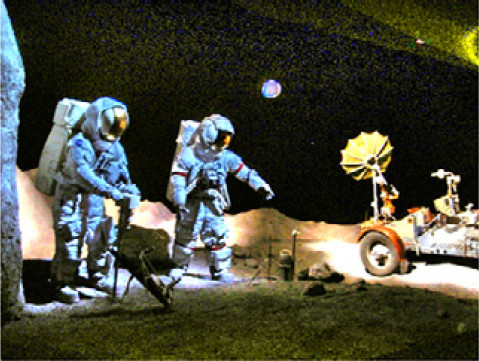
\includegraphics[width=\linewidth]{picture/LLIE/LLME1}
					\captionsetup{font=scriptsize}
					\label{fig: LLME1}
				\end{subfigure}
				\begin{subfigure}{0.24\textwidth}
					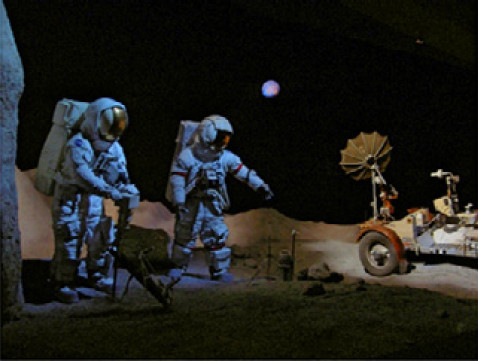
\includegraphics[width=\linewidth]{picture/LLIE/SRIE1}
					\captionsetup{font=scriptsize}
					\label{fig: SRIE1}	
				\end{subfigure}
				\begin{subfigure}{0.24\textwidth}
					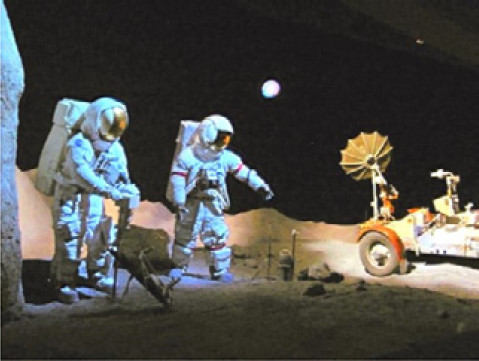
\includegraphics[width=\linewidth]{picture/LLIE/Our1}
					\captionsetup{font=scriptsize}
					\label{fig: Our1}	
				\end{subfigure} \\
				
				\begin{subfigure}{0.24\textwidth}
					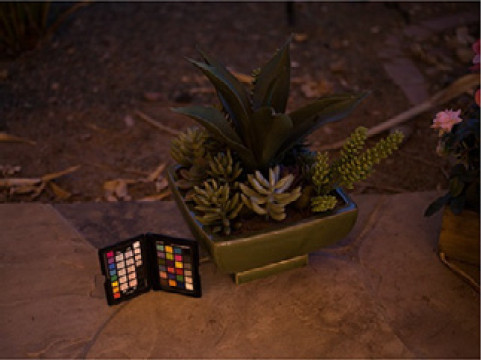
\includegraphics[width=\linewidth]{picture/LLIE/Input2}
					\captionsetup{font=scriptsize}
					\caption{Input}
					\label{fig: Input2}
				\end{subfigure}
				\begin{subfigure}{0.24\textwidth}
					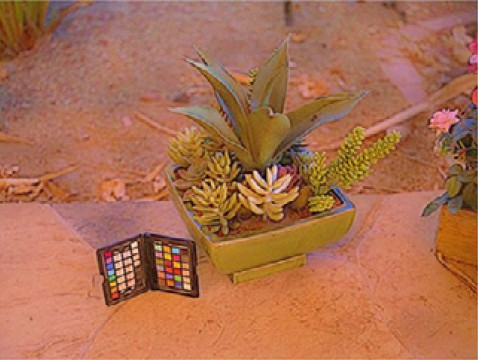
\includegraphics[width=\linewidth]{picture/LLIE/LLME2}
					\captionsetup{font=scriptsize}
					\caption{LLME}
					\label{fig: LLME2}
				\end{subfigure}
				\begin{subfigure}{0.24\textwidth}
					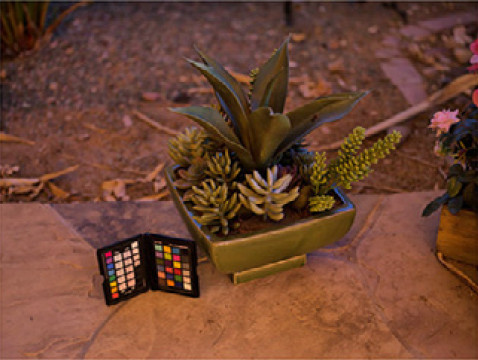
\includegraphics[width=\linewidth]{picture/LLIE/SRIE2}
					\captionsetup{font=scriptsize}
					\caption{SRIE}
					\label{fig: SRIE2}	
				\end{subfigure}
				\begin{subfigure}{0.24\textwidth}
					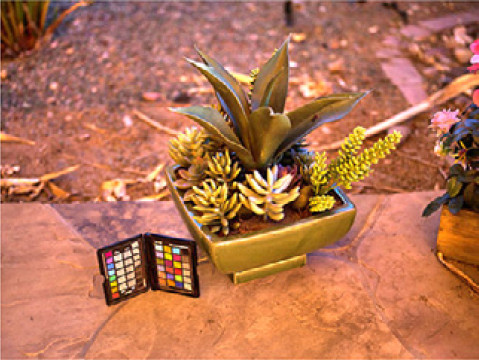
\includegraphics[width=\linewidth]{picture/LLIE/Our2}
					\captionsetup{font=scriptsize}
					\caption{Our}
					\label{fig: Our2}	
				\end{subfigure}
				\captionsetup{font=scriptsize}
				\caption{
					\label{fig: Examples of LLIE}
					Examples of low-light image enhanced results. The proposed method can not only improve the contrast of the image but also suppress the noise and artifacts in the dark regions. LIME generates color distorted results and causes noise amplification. SRIE generates under-enhancement results.
				}
			\end{figure}
			
			除了对比度,低光图像的另一个特殊退化是噪声。许多方法利用附加的去噪方法进行预处理或后处理。但是,采用去噪方法进行预处理会从产生模糊,而采用去噪方法进行处理则会产生噪声放大。因此,弱光图像增强还有很大的空间。
			
			\subsubsection{Contribution}
			
			\begin{itemize}
				\item[(1)] 
				作者提出了一种新颖的全卷积神经网络用于弱光图像增强(该网络的设计建立在 Retinex 理论基础之上)。
				
				\item[(2)]
				不同于以往使用附加去噪方法或附加去噪模块进行噪声抑制的方法,作者提出了一种新的频域噪声抑制损失,在分解时抑制反射图中的噪声。
				
				\item[(3)]
				在合成图像和真实低光图像上的实验结果表明,作者的方法在很大程度上优于当前的方法。结果表明,该方法可以有效提高光照不足条件下的人脸检测性能。				
			\end{itemize}	
				
			\subsubsection{Approach}
			
			\begin{figure}[htbp]
				% read manual to see what [ht] means and for other possible options
				\centering 
				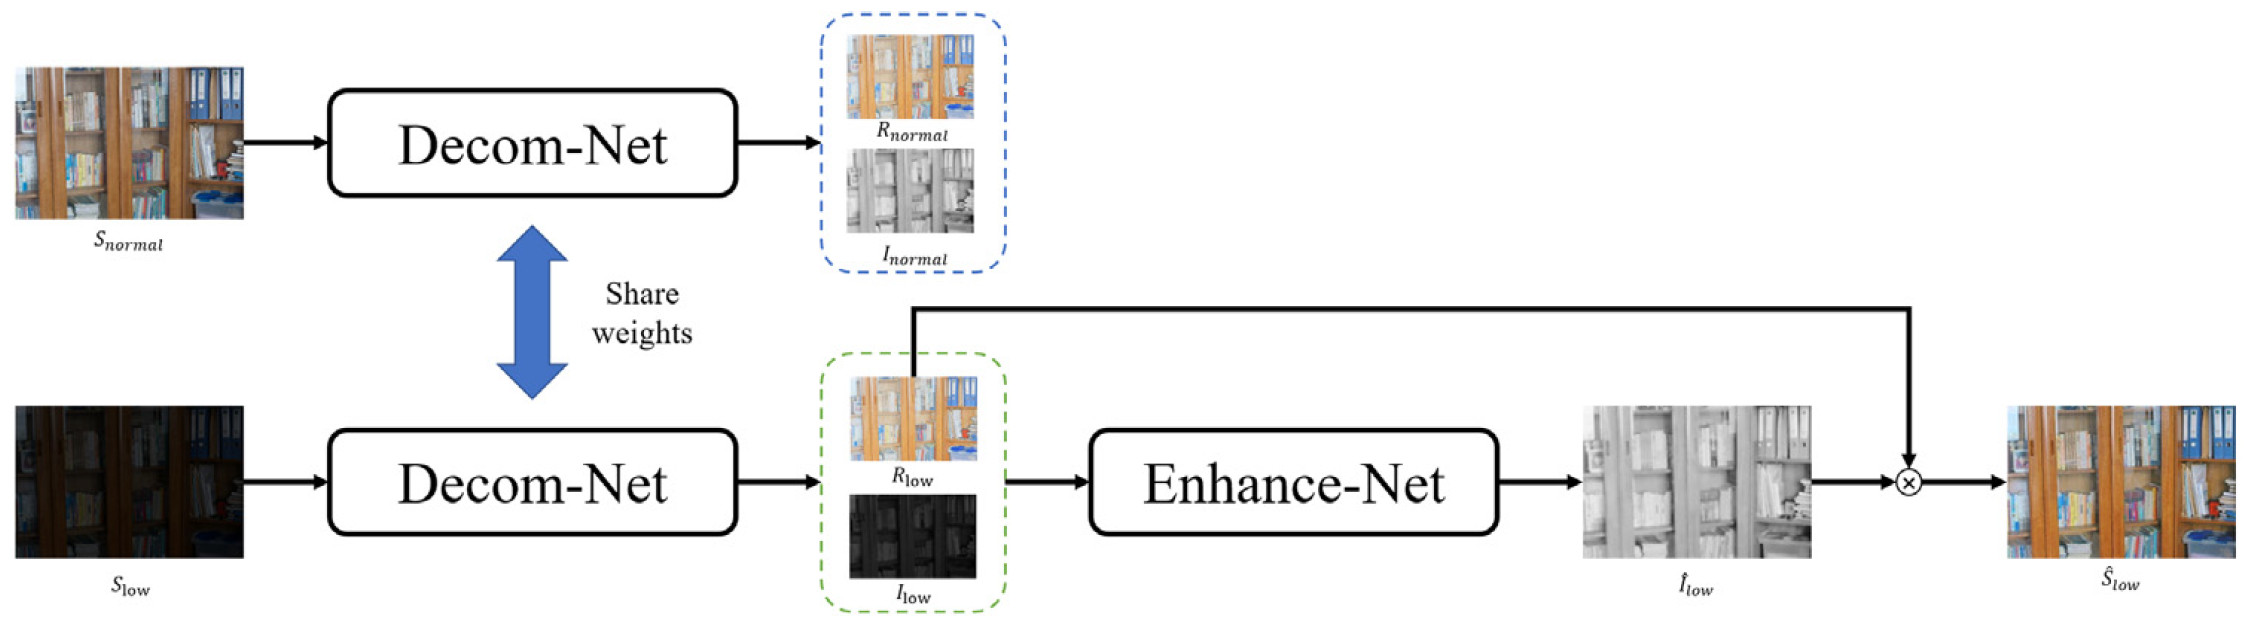
\includegraphics[width=\columnwidth]{picture/LLIE/Advanced RetinexNet}
				%\captionsetup{font=scriptsize}
				\caption{
					\label{fig: Advanced RetinexNet} 
					The overall network architecture of our proposed method.
				}
			\end{figure}
			
			该全卷积神经网络(Fig. \ref{fig: Advanced RetinexNet})包括两个子网:Decom-Net 和 Enhance-Net(Fig. \ref{fig: Decom-Net}与Fig. \ref{fig: Enhance-Net})。
			
			\begin{figure}[htbp]
				% read manual to see what [ht] means and for other possible options
				\centering 
				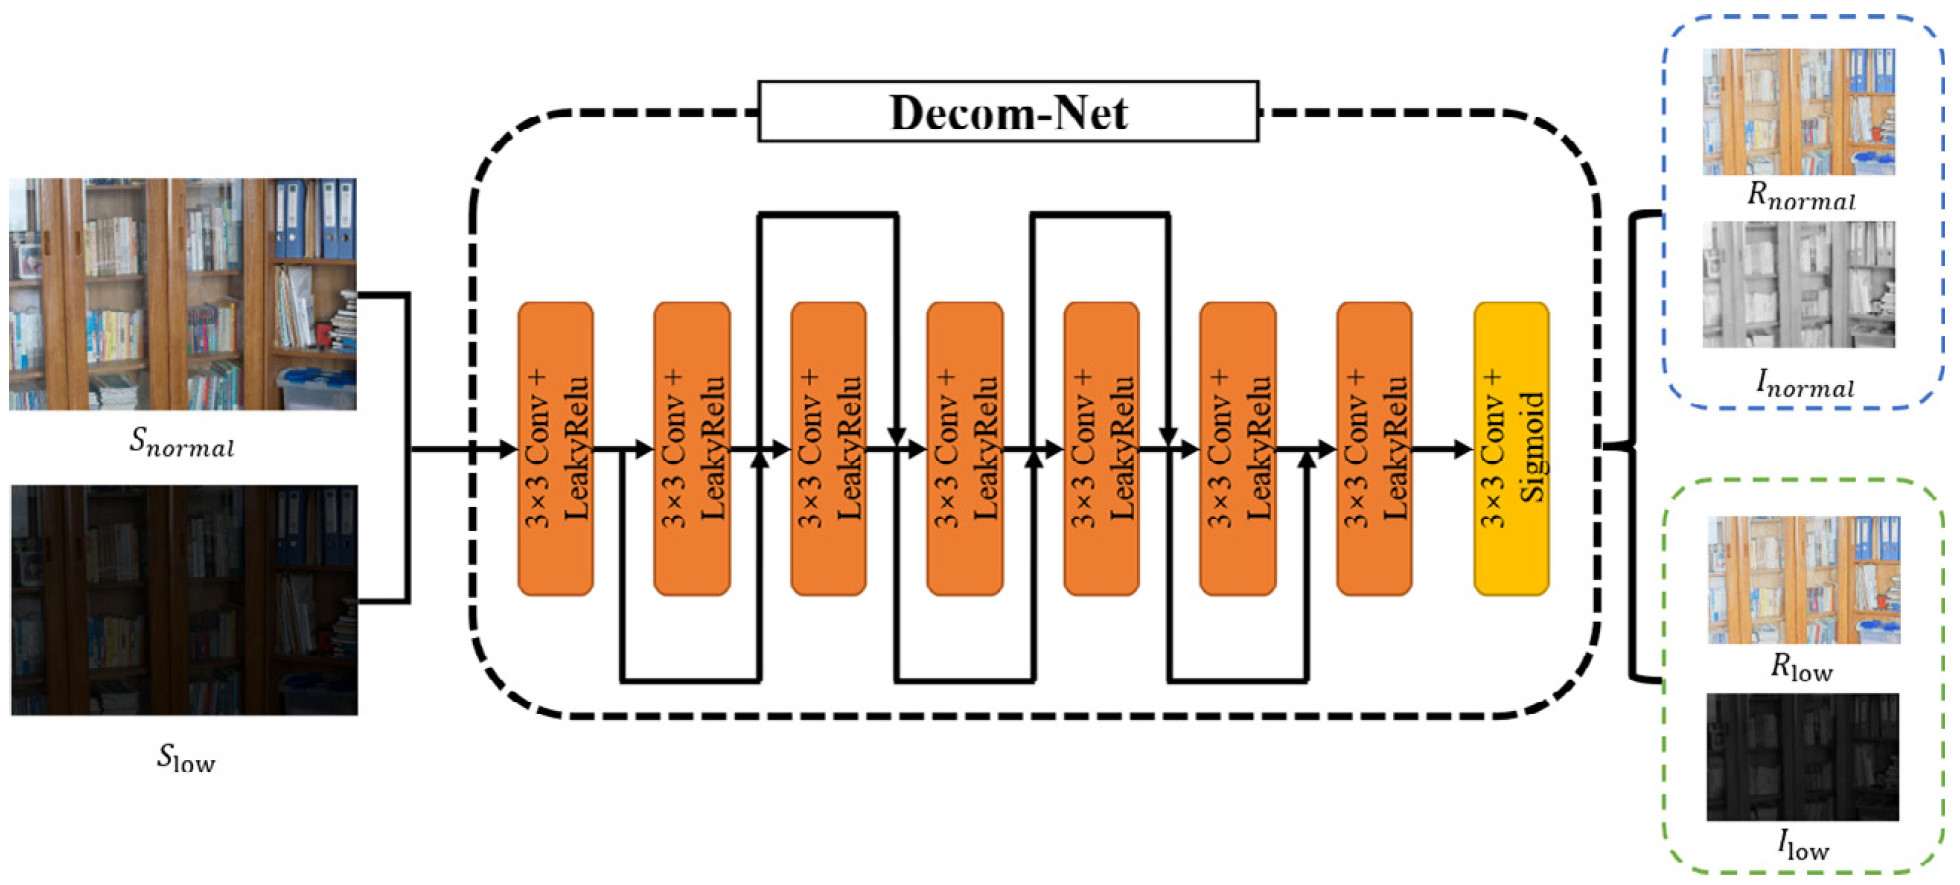
\includegraphics[width=0.8\columnwidth]{picture/LLIE/Decom-Net}
				%\captionsetup{font=scriptsize}
				\caption{
					\label{fig: Decom-Net} 
					The proposed Decom-Net architecture. The Decom-Net decomposes the input image into reflectance and illumination and can suppress the noise in the reflectance map.
					Note that the decompositions of normal-light images do not participate in the Enhance-Net training stage.
				}
			\end{figure}
			
			\begin{figure}[htbp]
				% read manual to see what [ht] means and for other possible options
				\centering 
				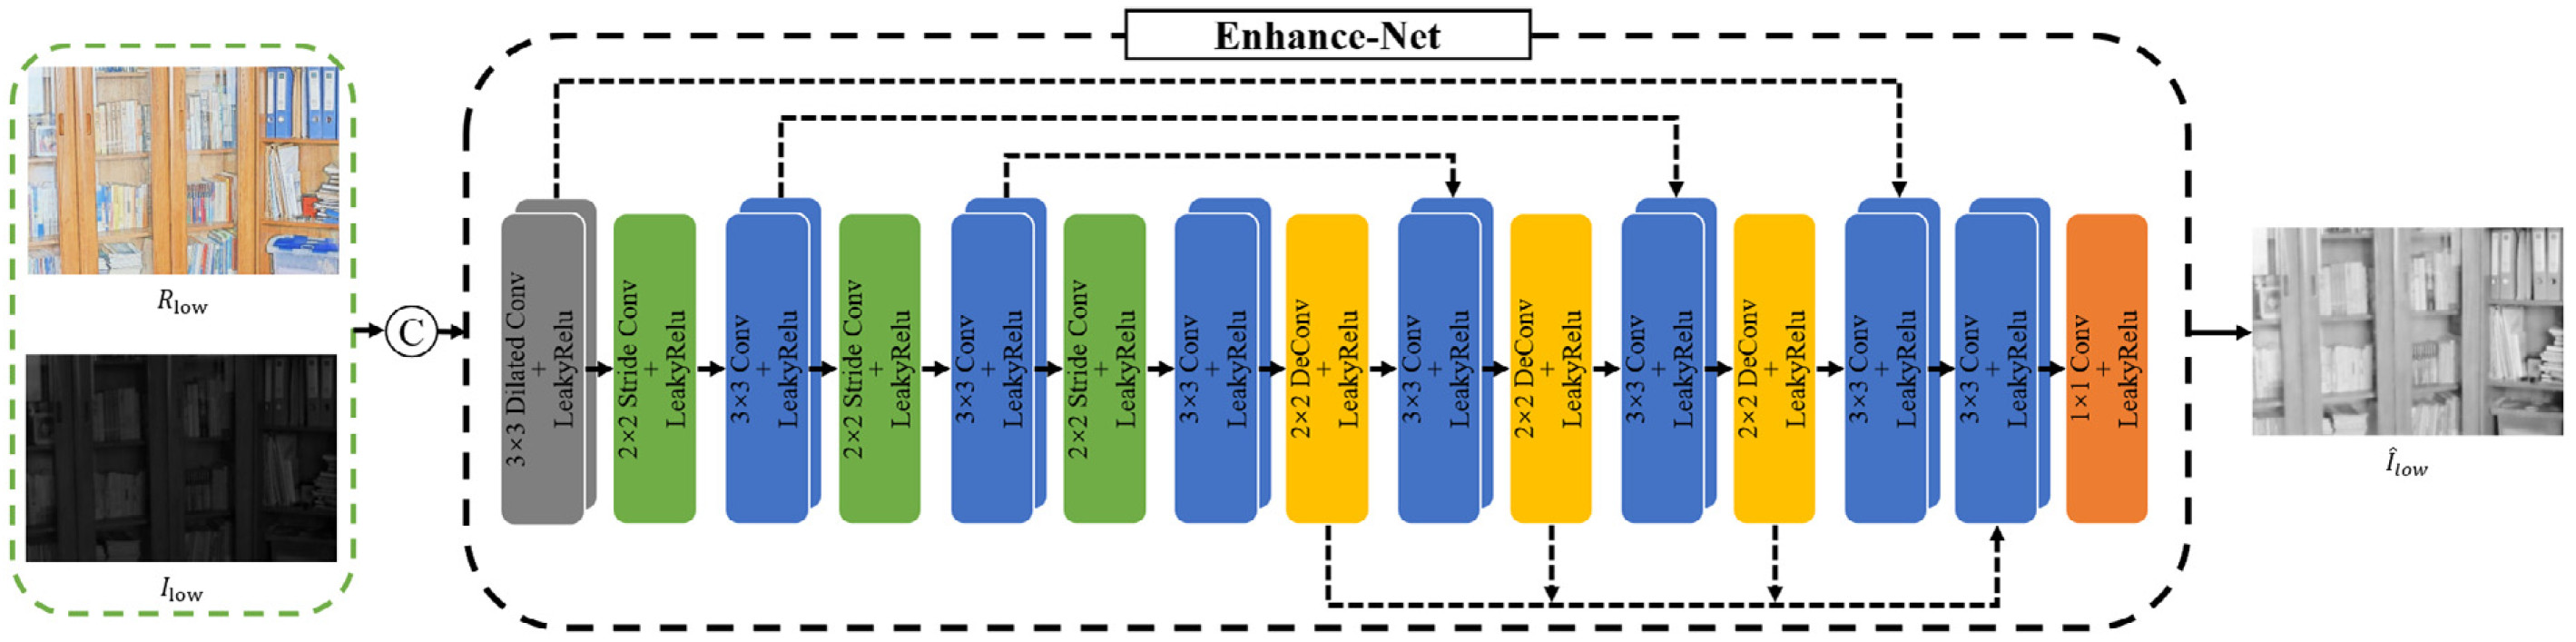
\includegraphics[width=\columnwidth]{picture/LLIE/Enhance-Net}
				%\captionsetup{font=scriptsize}
				\caption{
					\label{fig: Enhance-Net} 
					The proposed Enhance-Net architecture. The Enhance-Net takes the output of Decom-Net as the input to enhance the contrast and brightness of the illumination.
				}
			\end{figure}
			
			\begin{itemize}
				\item[(1)] 
				Decom-Net 将输入的低光图像分解为照度和反射率。
				
				\item[(2)]
				Enhance-Net 将 Decom-Net 的输出作为输入,通过精心设计的 "Deep-Narrow" ResUnet结构来提高光照对比度,该结构可以堆叠更多的层以获得更好的非线性建模能力,并且与常用的 U-Net 相比具有显著的参数缩减。
				
				\item[(3)]
				将 Decom-Net 的反射率与 Enhance-Net 的照度相结合,得到增强结果。通过设计良好的网络和合理的损失函数设置,作者的方法可以在适当增强图像对比度的同时实现对噪声的抑制。
			\end{itemize}	
			
			\subsubsection{Future}
			
			-
			
		\subsection{(2023.1)LightingNet: An Integrated Learning Method for Low-Light Image Enhancement}
		
		\paragraph{LightingNet:一种用于弱光图像增强的集成学习方法}
		
		\paragraph{(IEEE Transactions on Computational Imaging 二区) doi: 10.1109/TCI.2023.3240087}
		
			\subsubsection{Research Background}
			
			大多数基于 Retinex 的深度学习方法在弱光增强任务中表现出了更强的性能。然而,大多数深度学习方法再增强过程中仍然无法平衡噪声控制和增亮精度。大多数现有的弱光图像增强方法中存在的噪声、色差和细节失真等问题,为此,作者提出了一种集成学习方法 (LightingNet) 用于弱光图像增强。
			
			\subsubsection{Contribution}
			
			\subsubsection{Approach}
			
			LighingNet 由两个核心部分组成:
			
			\begin{itemize}
				\item[(1)] 
				互补学习子网;
				
				\item[(2)]
				The Vision Transformer (ViT) 弱光增强子网。ViT 弱光增强子网络通过全尺度架构学习拟合当前数据提供局部高级特征,利用互补学习子网络通过学习迁移提供全局微调特征。
			\end{itemize}	
			
			\subsubsection{Future}
			
			-
		
%	\begin{table}[!htbp]
%		\centering
%		\small
%		\caption{\label{tab: Datasets comparison}
%			Comparison between classic LLIE datasets
%			and our UHD-LL dataset. ‘Number’: the number of
%			paired images. ‘Resolution’: the average resolution of the
%			dataset. ‘Noise’: low-light images contain noise. ‘Real’:
%			both low-light images and GT are acquired in real scenes.} %表格的标题
%		%\resizebox{\textwidth}{!}{ %按照宽度调整调整表格大小
%			\begin{tabular}{>{\centering\arraybackslash}m{2.6cm}|c|c|c|c}
%				
%				\hline
%				
%				\textbf{Dataset} & \textbf{Number} & \textbf{Resolution} & \textbf{Noise} & \textbf{Real} \\
%				
%				\hline
%				
%				SID(RAW) & 5094 & \makecell{4240 $\times$ 2832 \\ 6000 $\times$ 4000} & \checkmark & \checkmark \\ 
%				MIT-Adobe FiveK & 5000 & 4000 $\times$ 2500 &  &  \\ 
%				Exposure-Errors  & 24000 & 1000 $\times$ 900 &  &  \\
%				LOL & 500/789 & 600 $\times$ 400 & \checkmark & \checkmark \\
%				\textbf{UHD-LL(Ours)} & \textbf{2150} & \textbf{3840 $\times$ 2160} & \checkmark & \checkmark \\
%				
%				\hline
%				
%			\end{tabular}
%			%}
%		\captionsetup{font=scriptsize} %设置标题字体与表格字体一致
%	\end{table}
	
%	\part{Unity VR 开发计划}
%
%		\section{项目需求}
%	
%			\subsection{主菜单界面开发}
%	
%			\begin{figure}[htbp]
%				% read manual to see what [ht] means and for other possible options
%				\centering 
%				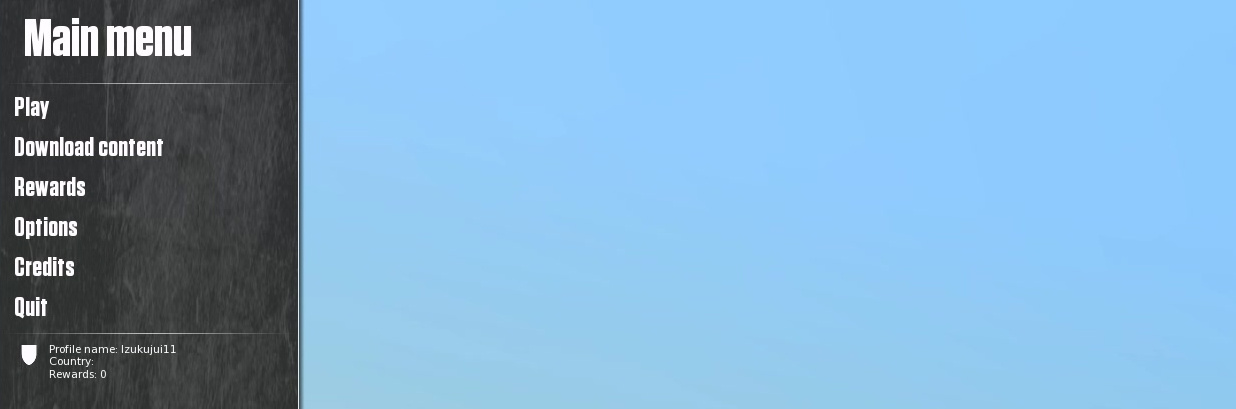
\includegraphics[width=\columnwidth]{picture/Main menu}
%				%\captionsetup{font=scriptsize}
%				\caption{
%					\label{fig: Main menu} 
%					主菜单界面。
%				}
%			\end{figure}
%			
%			启动进入游戏界面,随后进入游戏主菜单,主菜单至少需要包含 \textbf{Play},\textbf{Options}, \textbf{Quit}, 可以包含 \textbf{Credits} 和 \textbf{Rewards}。
%			
%				\subsubsection{Play}
%				
%				\begin{figure}[htbp]
%					% read manual to see what [ht] means and for other possible options
%					\centering 
%					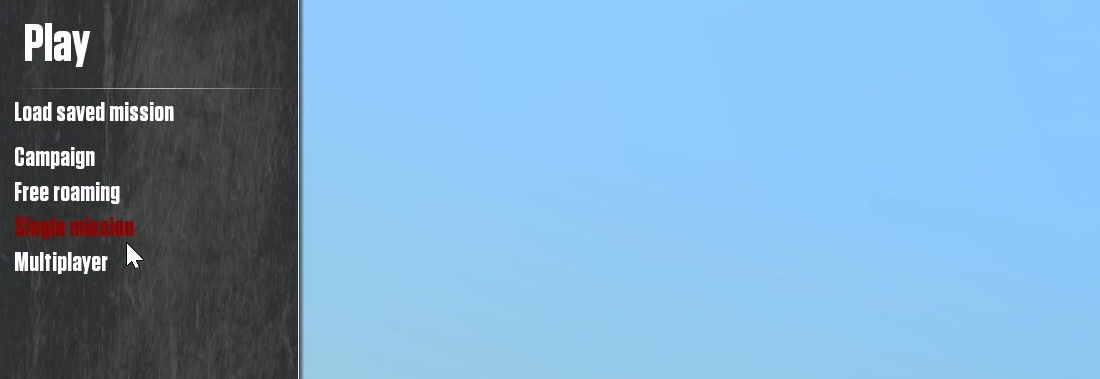
\includegraphics[width=\columnwidth]{picture/Play}
%					%\captionsetup{font=scriptsize}
%					\caption{
%						\label{fig: Play} 
%						\textbf{Play} 菜单界面。
%					}
%				\end{figure}
%				
%				通过射线选择 \textbf{Play} 进入 \textbf{Play} 菜单,\textbf{Play} 菜单至少需要包含 \textbf{Free roaming}, 可以包含 \textbf{Campaign}, \textbf{Single mission}, \textbf{Load saved mission}。玩家通过射线,选择不同的选项进入不同的游戏模式。
%				
%				\paragraph{Free roaming} 
%				
%				\textbf{Free roaming} 游戏模式赋予玩家极大的游戏自由度,进入该模式之后,玩家可以选择不同的船只与地图,同时自定义不同的海况;
%				
%				\paragraph{Campaign}
%				
%				-
%				
%				\paragraph{Single mission}
%				
%				-
%				
%				\paragraph{Multiplayer}
%				
%				-
%				
%				\paragraph{Load saved mission}
%				
%				-
%				
%				\subsubsection{Options}
%				
%					\paragraph{Controls}
%					
%					\begin{figure}[htbp]
%						% read manual to see what [ht] means and for other possible options
%						\centering 
%						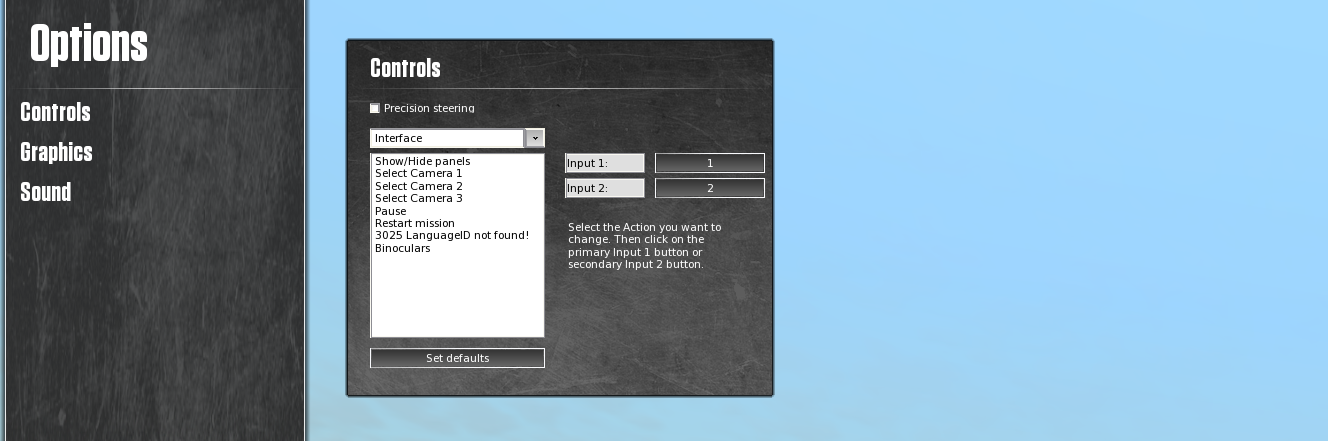
\includegraphics[width=\columnwidth]{picture/Options_Controls}
%						%\captionsetup{font=scriptsize}
%						\caption{
%							\label{fig: Options_Controls} 
%							\textbf{Controls} 选项界面。
%						}	
%					\end{figure}
%					
%					\textbf{Controls} 可以设置不同的控制模式,一种是对船面板的控制(第一人称视角),如Fig. \ref{fig: First-person perspective}所示。;另一种是以(第三人称视角)对船进行控制,并实现多种不同的第三人称视角,即多个 Camera ;最后是可以对船的控制进行自定义控制,如引擎推动开关和方向控制键。
%					
%					\begin{figure}[htbp]
%						% read manual to see what [ht] means and for other possible options
%						\centering
%						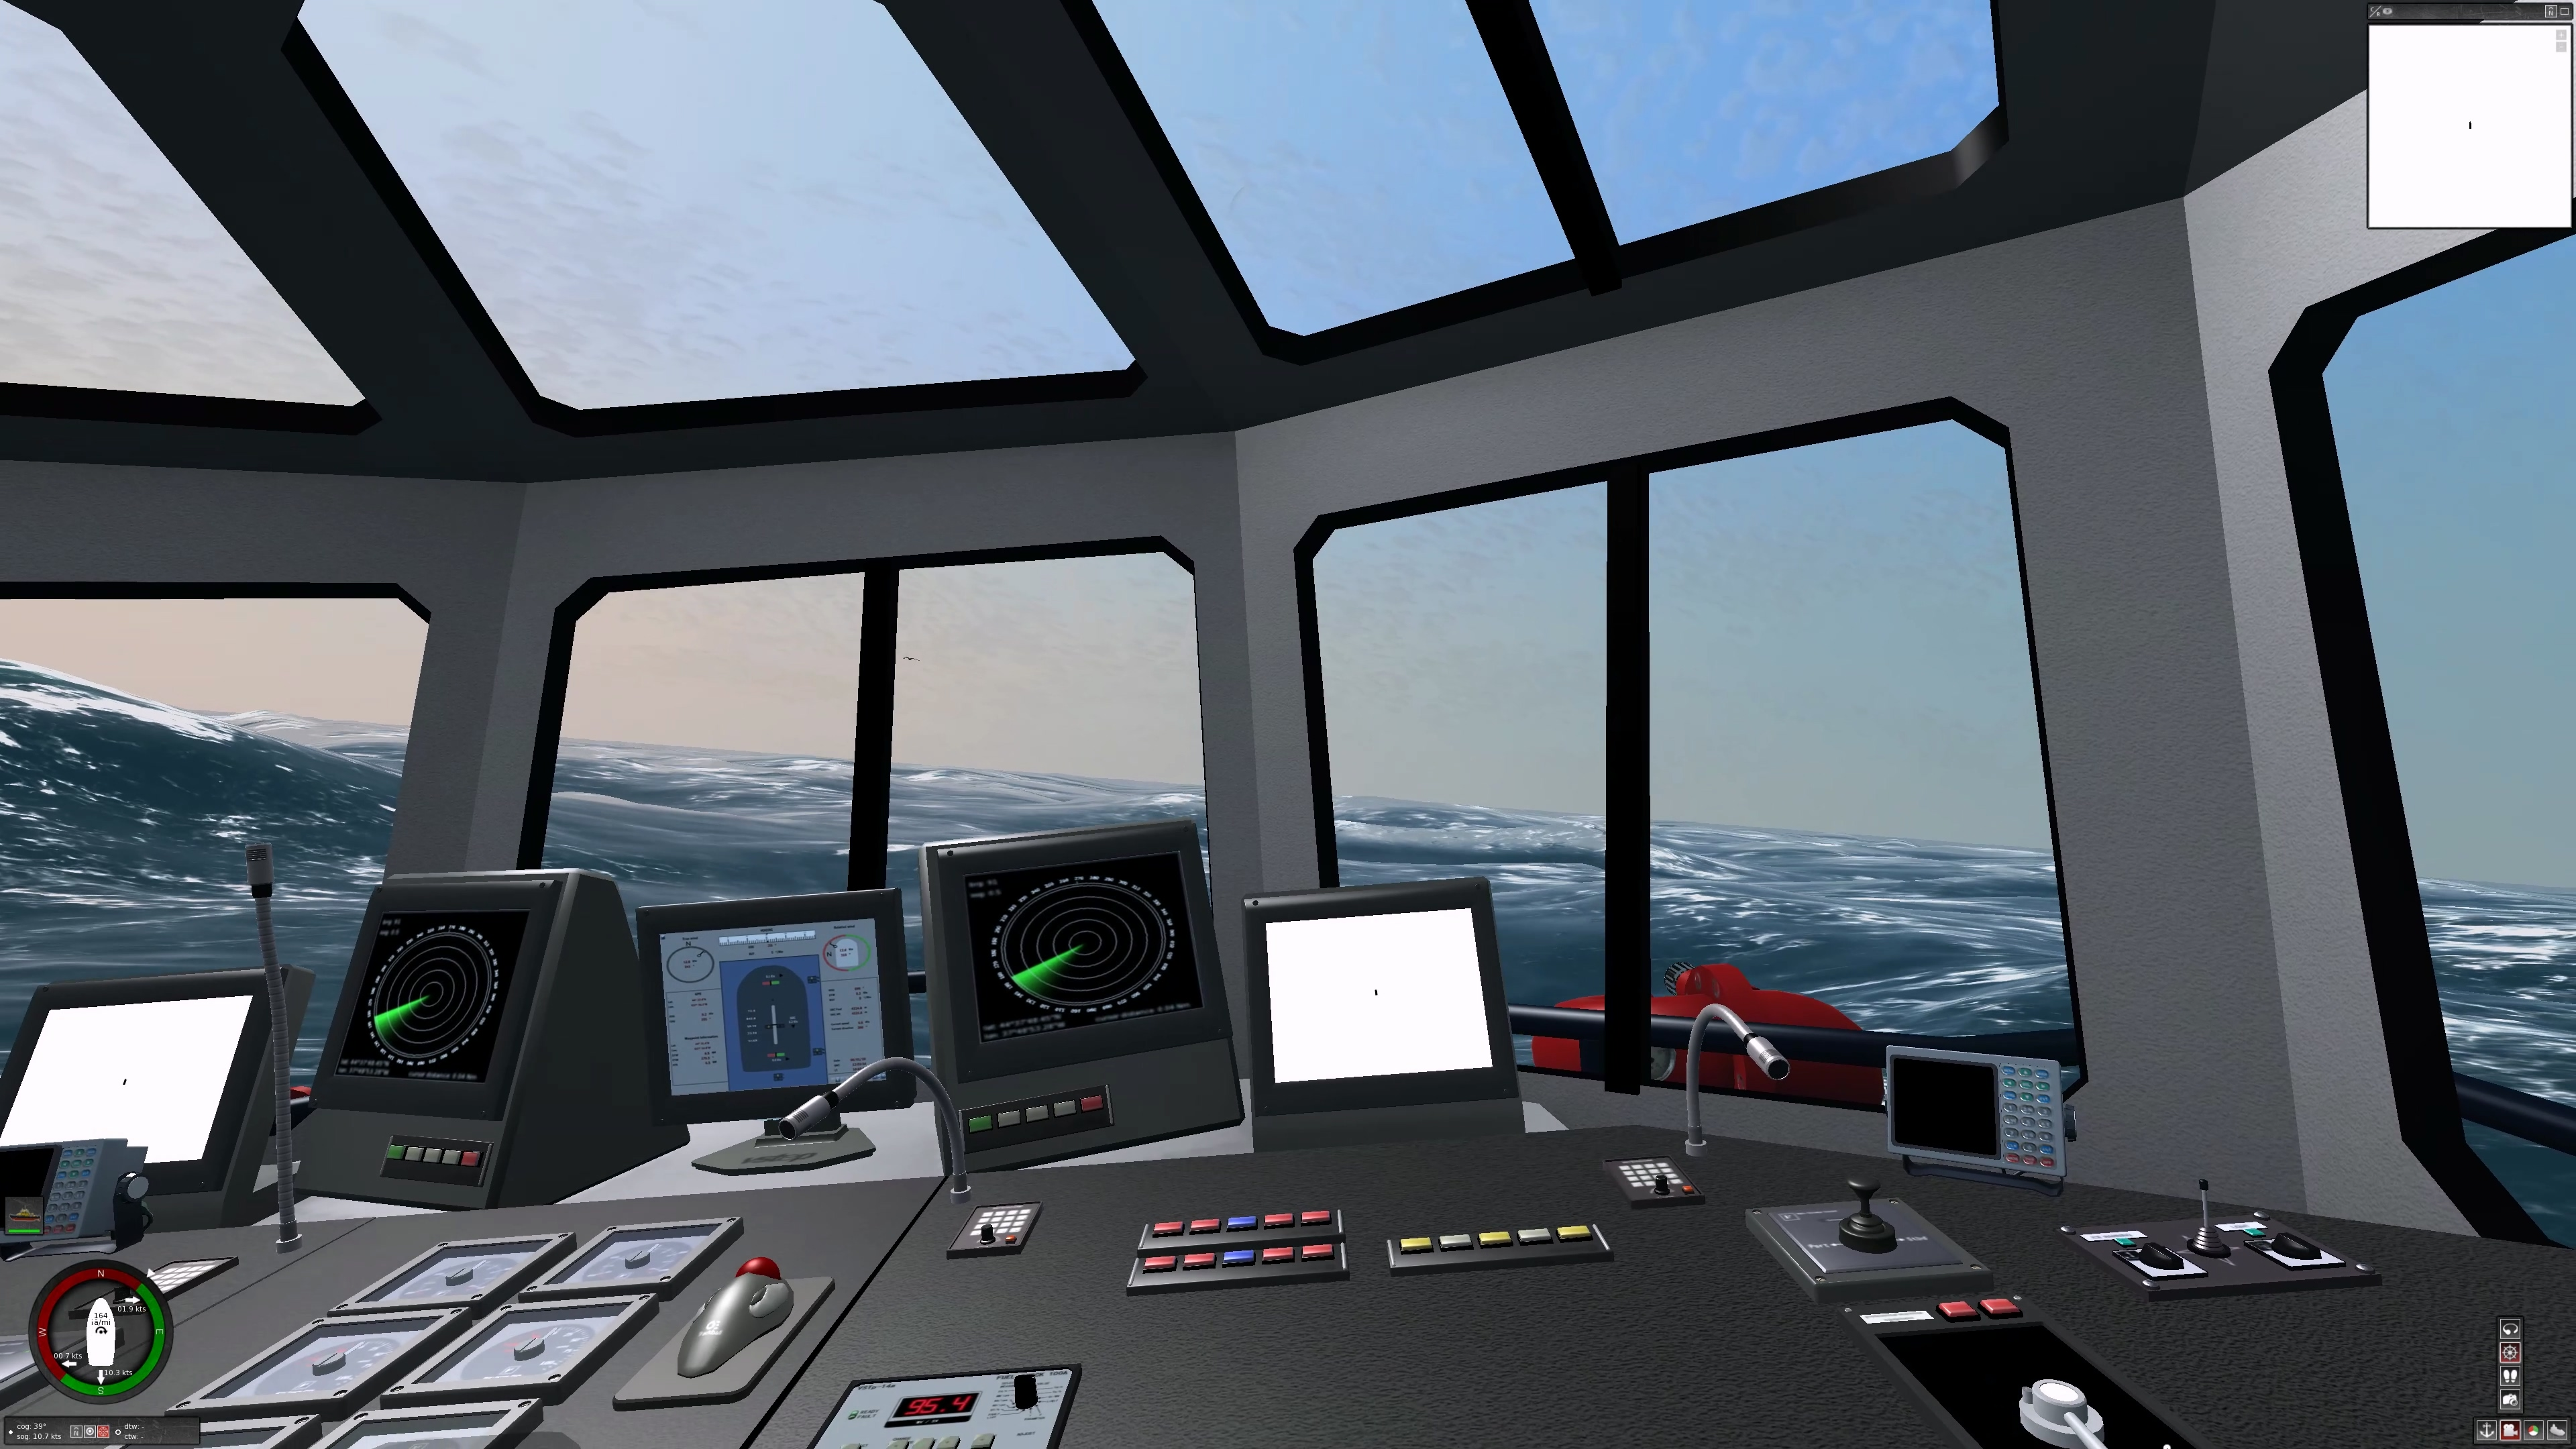
\includegraphics[width=\columnwidth]{picture/First-person perspective}
%						%\captionsetup{font=scriptsize}
%						\caption{
%							\label{fig: First-person perspective} 
%							第一人称视角游玩。
%						}	
%					\end{figure}
%					
%					
%					\paragraph{Graphics}
%					
%					\begin{figure}[htbp]
%						% read manual to see what [ht] means and for other possible options
%						\centering 
%						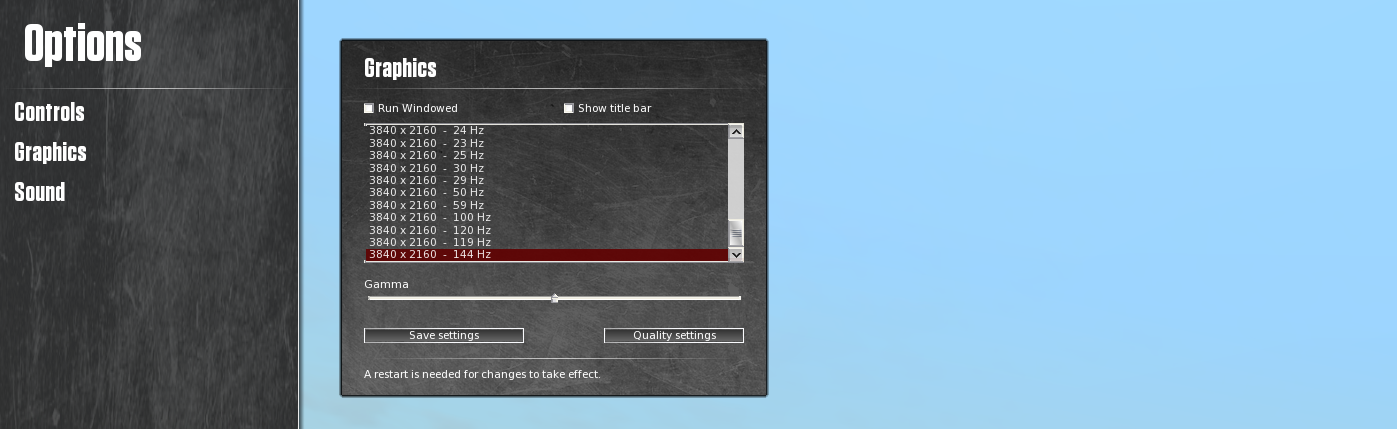
\includegraphics[width=\columnwidth]{picture/Options_Graphics}
%						%\captionsetup{font=scriptsize}
%						\caption{
%							\label{fig: Options_Graphics} 
%							\textbf{Graphics} 选项界面。
%						}	
%					\end{figure}
%					
%					\textbf{Graphics} 可以设置分辨率、是否窗口模式运行、设置刷新率和游戏渲染质量,并能够生成相应的保存的文件,每次启动时读取该保存文件。
%					
%					\paragraph{Sound}
%					
%					\begin{figure}[htbp]
%						% read manual to see what [ht] means and for other possible options
%						\centering 
%						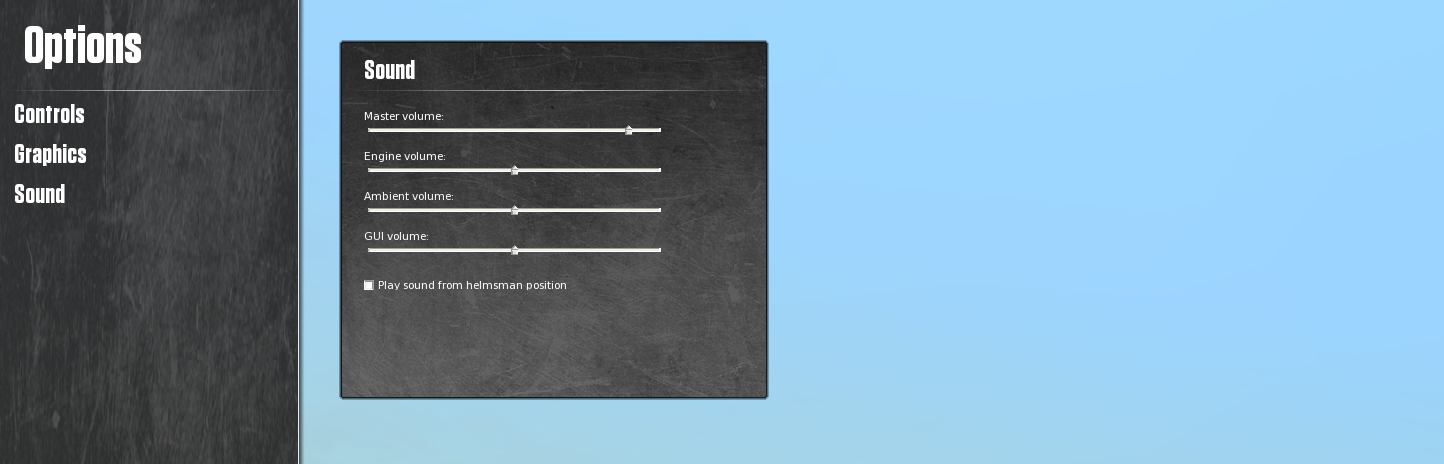
\includegraphics[width=\columnwidth]{picture/Options_Sound}
%						%\captionsetup{font=scriptsize}
%						\caption{
%							\label{fig: Options_Sound} 
%							\textbf{Sound} 选项界面。
%						}	
%					\end{figure}
%					
%					\textbf{Sound} 可以设置总音量(Master volume)、船只引擎的音量(Engine volume)、环境音乐的音量(Ambient volume)、界面音量( GUI volume)
%				
%				\subsubsection{Quit}
%				
%				退出游戏,即终止游戏程序运行。
%				
%				\subsubsection{Credits}
%				
%				游戏信息的展示,在主界面的滚动显示,或者是弹窗显示均可。
%				
%				\subsubsection{Rewards}
%	
%				游戏的奖杯模式,需要建立相应的任务系统,完成相应的任务之后跳杯,获得的奖杯可以在此处显示。
%	
%			\subsection{游戏模式}
%	
%				\subsubsection{Free roaming}
%				
%				\paragraph{船只模型自定义}
%				
%				\begin{figure}[htbp]
%					% read manual to see what [ht] means and for other possible options
%					\centering 
%					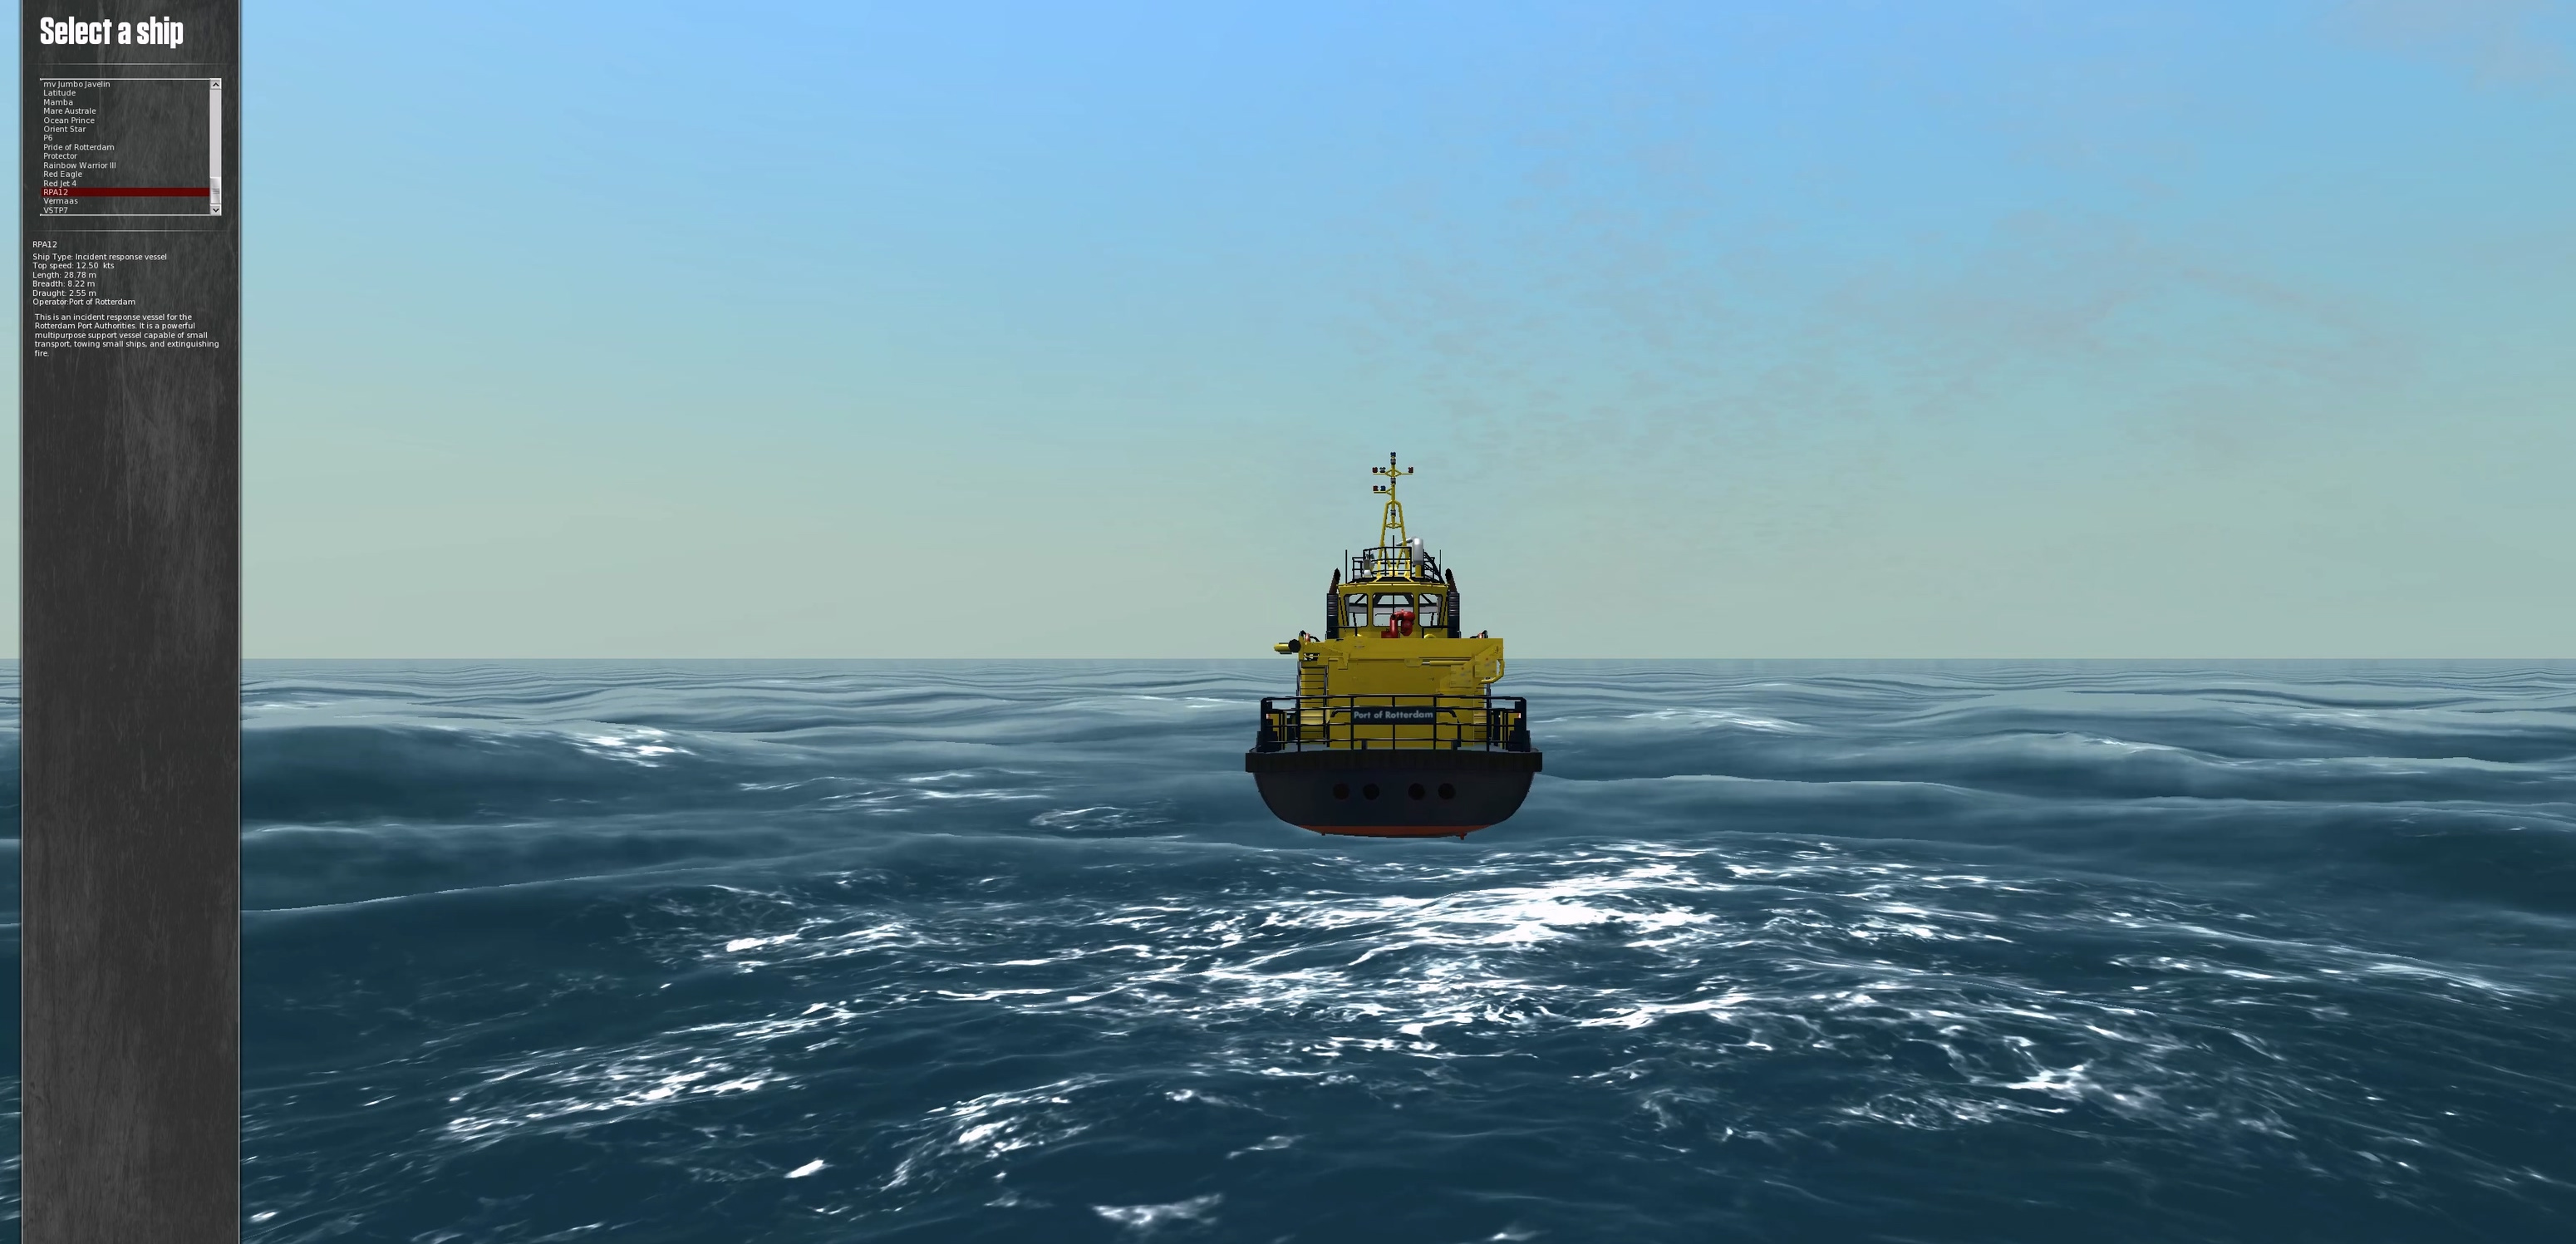
\includegraphics[width=\columnwidth]{picture/Select a ship}
%					%\captionsetup{font=scriptsize}
%					\caption{
%						\label{fig: Select a ship} 
%						船只模型选择界面。
%					}	
%				\end{figure}
%	
%				\textbf{Free roaming}下玩家可以任意进行船只选择,不同的船只会有不同的参数,如转向半径、平稳程度、马力、船只大小等会有明显区别。并且进行选择时,该船只会出现在主界面上,玩家可以直观的看到所选择的船只模型。
%				
%				\paragraph{环境自定义}
%				
%				\begin{figure}[htbp] 
%					% read manual to see what [ht] means and for other possible options
%					\centering 
%					% 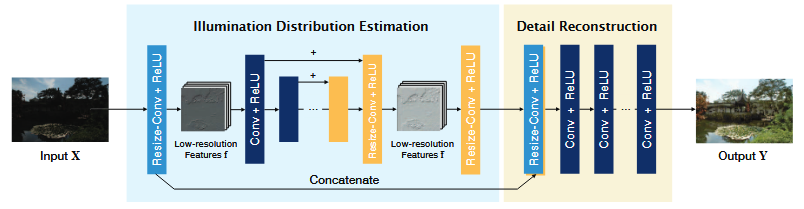
\includegraphics[width=0.8\columnwidth]{GLADNet}
%					
%					\begin{subfigure}{0.24\textwidth}
%						\includegraphics[width=\linewidth]{picture/Environment_Antarctic}
%						\captionsetup{font=scriptsize}
%						\caption{Antarctic}
%						\label{fig: Environment_Antarctic}
%					\end{subfigure}
%					\begin{subfigure}{0.24\textwidth}
%						\includegraphics[width=\linewidth]{picture/Environment_Atlantic Ocean}
%						\captionsetup{font=scriptsize}
%						\caption{Atlantic Ocean}
%						\label{fig: Environment_Atlantic Ocean}
%					\end{subfigure}
%					\begin{subfigure}{0.24\textwidth}
%						\includegraphics[width=\linewidth]{picture/Environment_Bora Bora}
%						\captionsetup{font=scriptsize}
%						\caption{Bora Bora}
%						\label{fig: Environment_Bora Bora}	
%					\end{subfigure}
%					\begin{subfigure}{0.24\textwidth}
%						\includegraphics[width=\linewidth]{picture/Environment_Dover}
%						\captionsetup{font=scriptsize}
%						\caption{Dover}
%						\label{fig: Environment_Dover}	
%					\end{subfigure} \\
%
%					\begin{subfigure}{0.24\textwidth}
%						\includegraphics[width=\linewidth]{picture/Environment_Hamburg}
%						\captionsetup{font=scriptsize}
%						\caption{Hamburg}
%						\label{fig: Environment_Hamburg}
%					\end{subfigure}
%					\begin{subfigure}{0.24\textwidth}
%						\includegraphics[width=\linewidth]{picture/Environment_Marseille}
%						\captionsetup{font=scriptsize}
%						\caption{Marseille}
%						\label{fig: Environment_Marseille}
%					\end{subfigure}
%					\begin{subfigure}{0.24\textwidth}
%						\includegraphics[width=\linewidth]{picture/Environment_New York}
%						\captionsetup{font=scriptsize}
%						\caption{New York}
%						\label{fig: Environment_New York}	
%					\end{subfigure}
%					\begin{subfigure}{0.24\textwidth}
%						\includegraphics[width=\linewidth]{picture/Environment_Padstow, Cornwall}
%						\captionsetup{font=scriptsize}
%						\caption{Padstow, Cornwall}
%						\label{fig: Environment_Padstow, Cornwall}	
%					\end{subfigure} \\
%
%					\begin{subfigure}{0.24\textwidth}
%						\includegraphics[width=\linewidth]{picture/Environment_Port of Rotterdam}
%						\captionsetup{font=scriptsize}
%						\caption{Port of Rotterdam}
%						\label{fig: Environment_Port of Rotterdam}
%					\end{subfigure}
%					\begin{subfigure}{0.24\textwidth}
%						\includegraphics[width=\linewidth]{picture/Environment_San Francisco}
%						\captionsetup{font=scriptsize}
%						\caption{San Francisco}
%						\label{fig: Environment_San Francisco}
%					\end{subfigure}
%					\begin{subfigure}{0.24\textwidth}
%						\includegraphics[width=\linewidth]{picture/Environment_Sydney}
%						\captionsetup{font=scriptsize}
%						\caption{Sydney}
%						\label{fig: Environment_Sydney}	
%					\end{subfigure}
%					\begin{subfigure}{0.24\textwidth}
%						\includegraphics[width=\linewidth]{picture/Environment_The Solent}
%						\captionsetup{font=scriptsize}
%						\caption{The Solent}
%						\label{fig: Environment_The Solent}	
%					\end{subfigure}
%					
%					\captionsetup{font=scriptsize}
%					\caption{
%						\label{fig: Environment selection}
%						在 \textbf{Free roaming} 下,玩家可以在Environment界面中自定义来自世界各地的海面环境。
%					}
%				\end{figure}
%				
%				此外,在不同的地图场景下,可以自定义船只起始出发的地点。如Fig. \ref{fig: Starting point selection}所示,在 New York 港口一共可以选择9个出发点,开始自由航行。
%				
%				\begin{figure}[htbp]
%					% read manual to see what [ht] means and for other possible options
%					\centering 
%					\includegraphics[width=\columnwidth]{picture/Starting point selection}
%					%\captionsetup{font=scriptsize}
%					\caption{
%						\label{fig: Starting point selection} 
%						在纽约港口环境下,船只出发地点选择。
%					}	
%				\end{figure}
%				
%				\paragraph{天气自定义}
%				
%				\begin{figure}[htbp]
%					% read manual to see what [ht] means and for other possible options
%					\centering 
%					\includegraphics[width=\columnwidth]{picture/Weather}
%					%\captionsetup{font=scriptsize}
%					\caption{
%						\label{fig: Weather} 
%						天气自定义界面。
%					}	
%				\end{figure}
%				
%				\textbf{Free roaming}下玩家也可以自定义各类海洋天气,以实现不同海况下的航行。可以设置不同的 \textbf{Temperature}、\textbf{Precipitation}、 \textbf{Wind speed}、 \textbf{Wind direction} 等参数,来实现不同的海况。
%				
%				
%				主要参数有6种,每一种的定义如下:
%				\begin{itemize}
%					\item [(1)] 
%					\textbf{Temperature} 设置4个类别,共60个等级,其中 Freezing $[-20 \sim -1]$、Cold $[0 \sim 9]$、Moderate $[10 \sim 19]$、Warm $[20 \sim 29]$、Hot $[30 \sim 40]$,单位为摄氏度。
%					
%					\item [(2)]
%					\textbf{Precipitation} 设置5个等级,其中分别为 Dry, Drizzle, Rain, Heavy Rain, Cloudburst。
%					
%					\item [(3)]
%					\textbf{Wind speed} 设置13个等级,其中分别为 Calm, Light air, Light breeze, Gentle breeze, Moderate breeze, Fresh breeze, Strong breeze, Moderate gale, Fresh gale, Strong gale, Storm, Violent Storm, Hurricane。
%					
%					\item [(4)]
%					\textbf{Wind direction} 设置16个方向,其中分别为 S, SSW, SW, WSW, W, WNW, NW, NNW, N, NNE, NE, ENE, E, ESE, SE, SSE, S。
%					
%					\item [(5)]
%					\textbf{Cloud Generation Settings} 设置3个类别,分别设置 Low Clouds, Middle Clouds, High Clouds;Low Clouds 的又分为3类,其中为 0 off, 1 Nimbostratus(乱层云) 2 Cumulonimbus(积雨云); Middle Clouds 分为3类,其中为 0 off, 1 Altostratus(高层云), 2 Altocumulus(高积云); High Clouds 分为3类,其中 0 off, 1 Cirrus(卷云), 2 Cirrocumulus(卷积云)
%					
%					\item [(6)]
%					\textbf{Fog Density} 则设置为 $0 \sim 100\%$,百分比越高,能见度越差。
%				\end{itemize}
%	
%				玩家除了可以自定义天气以外,需要快捷的辅助玩家设置不同类型的天气,故引入 \textbf{Preset} 设定。\textbf{Preset} 设置了9种天气,每一种天气对应上述6种参数不同的设定,如Fig. \ref{fig: Weather}所示。9种天气为 Clear sky, Drizzle(毛毛雨), Foggy, Hail(冰雹), Light snow, Rainy, Snow storm(暴风雪), Storm, Wind\footnote{在实际的开发中,只需要开发这9种对应的天气,如果对每一种参数搭配($60 \times 5 \times 13 \times 16 \times 9 \times 100$)都开发对应的天气,这样的话,开发成本会很大。如 Clear sky 对应 27 warm, Dry, Gentle breeze, Wind E, Cirrocumulus, Fog Density = 0\%}。
%				
%				\begin{figure}[ht] 
%					% read manual to see what [ht] means and for other possible options
%					\centering 
%					% \includegraphics[width=0.8\columnwidth]{GLADNet}
%					
%					\begin{subfigure}{0.3\textwidth}
%						\includegraphics[width=\linewidth]{picture/Clear sky}
%						\captionsetup{font=scriptsize}
%						\caption{Clear sky}
%						\label{fig: Clear sky}
%					\end{subfigure}
%					\begin{subfigure}{0.3\textwidth}
%						\includegraphics[width=\linewidth]{picture/Drizzle}
%						\captionsetup{font=scriptsize}
%						\caption{Drizzle}
%						\label{fig: Drizzle}
%					\end{subfigure}
%					\begin{subfigure}{0.3\textwidth}
%						\includegraphics[width=\linewidth]{picture/Foggy}
%						\captionsetup{font=scriptsize}
%						\caption{Foggy}
%						\label{fig: Foggy}	
%					\end{subfigure}\\
%					\begin{subfigure}{0.3\textwidth}
%						\includegraphics[width=\linewidth]{picture/Hail}
%						\captionsetup{font=scriptsize}
%						\caption{Hail}
%						\label{fig: Hail}	
%					\end{subfigure}
%					\begin{subfigure}{0.3\textwidth}
%						\includegraphics[width=\linewidth]{picture/Light snow}
%						\captionsetup{font=scriptsize}
%						\caption{Light snow}
%						\label{fig: Light snow}
%					\end{subfigure}
%					\begin{subfigure}{0.3\textwidth}
%						\includegraphics[width=\linewidth]{picture/Rainy}
%						\captionsetup{font=scriptsize}
%						\caption{Rainy}
%						\label{fig: Rainy}
%					\end{subfigure}\\
%					\begin{subfigure}{0.3\textwidth}
%						\includegraphics[width=\linewidth]{picture/Snow storm}
%						\captionsetup{font=scriptsize}
%						\caption{Snow storm}
%						\label{fig: Snow storm}	
%					\end{subfigure}
%					\begin{subfigure}{0.3\textwidth}
%						\includegraphics[width=\linewidth]{picture/Storm}
%						\captionsetup{font=scriptsize}
%						\caption{Storm}
%						\label{fig: Storm}	
%					\end{subfigure}
%					\begin{subfigure}{0.3\textwidth}
%						\includegraphics[width=\linewidth]{picture/Wind}
%						\captionsetup{font=scriptsize}
%						\caption{Wind}
%						\label{fig: Wind}
%					\end{subfigure}
%					\captionsetup{font=scriptsize}
%					\caption{
%						\label{fig: Weather}
%						9种不同的天气下的海况表现。
%					}
%				\end{figure}
%			
%				\paragraph{操作视角自定义}
%				
%				玩家在操纵船只时,可以自定义不同的操作视角,主要有三种游戏视角,一个自由视角,分别为 orbit(航线视角), helmsman(舵手视角), walkthrough(行人视角), photo camera mode, 如Fig. \ref{fig: View}所示。
%				
%				\begin{figure}[htbp] 
%					% read manual to see what [ht] means and for other possible options
%					\centering 
%					% \includegraphics[width=0.8\columnwidth]{GLADNet}
%					
%					\begin{subfigure}{0.45\textwidth}
%						\includegraphics[width=\linewidth]{picture/orbit}
%						\captionsetup{font=scriptsize}
%						\caption{orbit}
%						\label{fig: orbit}
%					\end{subfigure}
%					\begin{subfigure}{0.45\textwidth}
%						\includegraphics[width=\linewidth]{picture/helmsman}
%						\captionsetup{font=scriptsize}
%						\caption{Drizzle}
%						\label{fig: helmsman}
%					\end{subfigure}\\
%					\begin{subfigure}{0.45\textwidth}
%						\includegraphics[width=\linewidth]{picture/walkthrough}
%						\captionsetup{font=scriptsize}
%						\caption{Walkthrough}
%						\label{fig: walkthrough}	
%					\end{subfigure}
%					\begin{subfigure}{0.45\textwidth}
%						\includegraphics[width=\linewidth]{picture/photo camera mode}
%						\captionsetup{font=scriptsize}
%						\caption{photo camera mode}
%						\label{fig: photo camera mode}	
%					\end{subfigure}
%					\captionsetup{font=scriptsize}
%					\caption{
%						\label{fig: View}						
%						4种不同的操控视角。
%					}
%				\end{figure}

	%	\section{Analysis}
	
	%	In this section you will need to show your experimental results. Use tables and
	%	graphs when it is possible. Table~\ref{tbl:bins} is an example.
	
	%	\begin{table}[ht]
		%		\begin{center}
			%			\caption{Every table needs a caption.}
			%			\label{tbl:bins} % spaces are big no-no withing labels
			%			\begin{tabular}{|ccc|} 
				%				\hline
				%				\multicolumn{1}{|c}{$x$ (m)} & \multicolumn{1}{c|}{$V$ (V)} & \multicolumn{1}{c|}{$V$ (V)} \\
				%				\hline
				%				0.0044151 &   0.0030871 &   0.0030871\\
				%				0.0021633 &   0.0021343 &   0.0030871\\
				%				0.0003600 &   0.0018642 &   0.0030871\\
				%				0.0023831 &   0.0013287 &   0.0030871\\
				%				\hline
				%			\end{tabular}
			%		\end{center}
		%	\end{table}
	%	
	%	Analysis of equation~\ref{eq:aperp} shows ...
	%	
	%	Note: this section can be integrated with the previous one as long as you
	%	address the issue. Here explain how you determine uncertainties for different
	%	measured values. Suppose that in the experiment you make a series of
	%	measurements of a resistance of the wire $R$ for different applied voltages
	%	$V$, then you calculate the temperature from the resistance using a known
	%	equation and make a plot  temperature vs. voltage squared. Again suppose that
	%	this dependence is expected to be linear~\cite{Cyr}, and the proportionality coefficient
	%	is extracted from the graph. Then what you need to explain is that for the
	%	resistance and the voltage the uncertainties are instrumental (since each
	%	measurements in done only once), and they are $\dots$. Then give an equation
	%	for calculating the uncertainty of the temperature from the resistance
	%	uncertainty. Finally explain how the uncertainty of the slop of the graph was
	%	found (computer fitting, graphical method, \emph{etc}.)
	%	
	%	If in the process of data analysis you found any noticeable systematic
	%	error(s), you have to explain them in this section of the report.
	%	
	%	It is also recommended to plot the data graphically to efficiently illustrate
	%	any points of discussion. For example, it is easy to conclude that the
	%	experiment and theory match each other rather well if you look at
	%	Fig.~\ref{fig:samplesetup} and Fig.~\ref{fig:exp_plots}.
	%	
	%	\begin{figure}[ht] 
		%		\centering
		%		\includegraphics[width=0.5\columnwidth]{sr_squeezing_vs_detuning}
		%		
		%		% some figures do not need to be too wide
		%		\caption{
			%			\label{fig:exp_plots}  
			%			Every plot must have axes labeled.
			%		}
		%	\end{figure}
	
	
	%	\section{Conclusions}
	%	Here you briefly summarize your findings.
	
	%++++++++++++++++++++++++++++++++++++++++
	% References section will be created automatically 
	% with inclusion of "thebibliography" environment
	% as it shown below. See text starting with line
	% \begin{thebibliography}{99}
		% Note: with this approach it is YOUR responsibility to put them in order
		% of appearance.
		
		\renewcommand{\refname}{References}
		
		
		%	\begin{thebibliography}{00}
			
			%		\bibitem{b1}\label{cite:b1}
			%		W. Wang, C. Wei, W. Yang and J. Liu, "GLADNet: Low-Light Enhancement Network with Global Awareness," 2018 13th IEEE International Conference on Automatic Face \& Gesture Recognition (FG 2018), Xi'an, China, 2018, pp. 751-755, DOI: 10.1109/FG.2018.00118.
			
			%		\bibitem{b2}\label{cite:b2}
			%		A.\ Mahajan, K.\ Somaraj and M. Sameer, "Adopting Artificial Intelligence Powered ConvNet To Detect Epileptic Seizures," 2020 IEEE-EMBS Conference on Biomedical Engineering and Sciences (IECBES), Langkawi Island, Malaysia, 2021, pp. 427-432, DOI: 10.1109/IECBES48179.2021.9398832.
			
			%		\bibitem{Cyr}
			%		N.\ Cyr, M.\ T$\hat{e}$tu, and M.\ Breton,
			% "All-optical microwave frequency standard: a proposal,"
			%		IEEE Trans.\ Instrum.\ Meas.\ \textbf{42}, 640 (1993).
			
			
			
			%	\end{thebibliography}
		
		\bibliographystyle{unsrt}
		\bibliography{reference}
		
		
	\end{document}
